%%%%%%%%%%%%%%%%%%%%%%%%%%%%%%%%%%%%%%%%%%%%%%%%%%%%%%%%%%%%%%%%%%%%%%%%%%%%
% AGUJournalTemplate.tex: this template file is for articles formatted with LaTeX
%
% This file includes commands and instructions
% given in the order necessary to produce a final output that will
% satisfy AGU requirements, including customized APA reference formatting.
%
% You may copy this file and give it your
% article name, and enter your text.
%
% guidelines and troubleshooting are here: 

%% user added for convenience, can be removed before submission:



%% To submit your paper:
\documentclass[draft]{agujournal2019}
\usepackage{url} %this package should fix any errors with URLs in refs.
\usepackage{lineno}
\usepackage[inline]{trackchanges} %for better track changes. finalnew option will compile document with changes incorporated.
\usepackage{soul}

% MY OWN ADDED PACKAGES TO RENDER UNITS
\usepackage{gensymb}
\usepackage{booktabs}
\usepackage{siunitx}
\sisetup{separate-uncertainty=true}
\usepackage[section]{placeins}

\linenumbers
%%%%%%%
% As of 2018 we recommend use of the TrackChanges package to mark revisions.
% The trackchanges package adds five new LaTeX commands:
%
%  \note[editor]{The note}
%  \annote[editor]{Text to annotate}{The note}
%  \add[editor]{Text to add}
%  \remove[editor]{Text to remove}
%  \change[editor]{Text to remove}{Text to add}
%
% complete documentation is here: http://trackchanges.sourceforge.net/
%%%%%%%

\draftfalse

%% Enter journal name below.
%% Choose from this list of Journals:
%
% JGR: Atmospheres
% JGR: Biogeosciences
% JGR: Earth Surface
% JGR: Oceans
% JGR: Planets
% JGR: Solid Earth
% JGR: Space Physics
% Global Biogeochemical Cycles
% Geophysical Research Letters
% Paleoceanography and Paleoclimatology
% Radio Science
% Reviews of Geophysics
% Tectonics
% Space Weather
% Water Resources Research
% Geochemistry, Geophysics, Geosystems
% Journal of Advances in Modeling Earth Systems (JAMES)
% Earth's Future
% Earth and Space Science
% Geohealth
%
% ie, \journalname{Water Resources Research}

\journalname{JGR: Biogeosciences}


\begin{document}

%%%%%%%%%%%%%%%%%%%%%%%%%%%%%%%%%%%%%%%%%%%%%%%
%  TITLE
%
% (A title should be specific, informative, and brief. Use
% abbreviations only if they are defined in the abstract. Titles that
% start with general keywords then specific terms are optimized in
% searches)
%
%%%%%%%%%%%%%%%%%%%%%%%%%%%%%%%%%%%%%%%%%%%%%%%

% Example: \title{This is a test title}

\title{Reversible Regime Change: Climate-driven phytoplankton community shifts in the Cariaco Basin, Venezuela}

%%%%%%%%%%%%%%%%%%%%%%%%%%%%%%%%%%%%%%%%%%%%%%%
%
%  AUTHORS AND AFFILIATIONS
%
%%%%%%%%%%%%%%%%%%%%%%%%%%%%%%%%%%%%%%%%%%%%%%%

% Authors are individuals who have significantly contributed to the
% research and preparation of the article. Group authors are allowed, if
% each author in the group is separately identified in an appendix.)

% List authors by first name or initial followed by last name and
% separated by commas. Use \affil{} to number affiliations, and
% \thanks{} for author notes.
% Additional author notes should be indicated with \thanks{} (for
% example, for current addresses).

% Example: \authors{A. B. Author\affil{1}\thanks{Current address, Antartica}, B. C. Author\affil{2,3}, and D. E.
% Author\affil{3,4}\thanks{Also funded by Monsanto.}}

\authors{Benjamin Post\affil{1,2}, Esteban Acevedo-Trejos\affil{3}, Subhendu Chakraborty\affil{1}, Andrew D. Barton\affil{4}, Agostino Merico\affil{1,2,5}}


% \affiliation{1}{First Affiliation}
% \affiliation{2}{Second Affiliation}
% \affiliation{3}{Third Affiliation}
% \affiliation{4}{Fourth Affiliation}

\affiliation{1}{Systems Ecology Group, Leibniz Centre for Tropical Marine Research (ZMT), Bremen, Germany}
\affiliation{2}{School of Science, Constructor University, Bremen, Germany}
\affiliation{3}{Earth Surface Process Modelling, GFZ German Research Centre for Geosciences, Potsdam, Germany}
\affiliation{4}{Scripps Institution of Oceanography and Department of Ecology, Behavior and Evolution, University of California San Diego, La Jolla, CA, United States}
\affiliation{5}{Faculty of Biology and Chemistry, University of Bremen, Germany}
%(repeat as many times as is necessary)


% Corresponding author mailing address and e-mail address:

% (include name and email addresses of the corresponding author.  More
% than one corresponding author is allowed in this LaTeX file and for
% publication; but only one corresponding author is allowed in our
% editorial system.)

% Example: \correspondingauthor{First and Last Name}{email@address.edu}

\correspondingauthor{Benjamin Post}{benjaminpost@aoop.de}



%%%%%%%%%%%%%%%%%%%%%%%%%%%%%%%%%%%%%%%%%%%%%%%
% KEY POINTS
%%%%%%%%%%%%%%%%%%%%%%%%%%%%%%%%%%%%%%%%%%%%%%%
%  List up to three key points (at least one is required)
%  Key Points summarize the main points and conclusions of the article
%  Each must be 140 characters or fewer with no special characters or punctuation and must be complete sentences

% Example:
% \begin{keypoints}
% \item	List up to three key points (at least one is required)
% \item	Key Points summarize the main points and conclusions of the article
% \item	Each must be 140 characters or fewer with no special characters or punctuation and must be complete sentences
% \end{keypoints}

\begin{keypoints}
\item The CARIACO phytoplankton time series reveals two temporal clusters, linked to a 2004 shift from high to low upwelling and return in 2014.
\item Diversity metrics show no significant difference except lower turnover and higher evenness during the cluster with low upwelling conditions.
\item Gradient forest analysis finds AMO index as strongest predictor of community shifts, highlighting large-scale climate impacts on ecosystem.
\end{keypoints}

%%%%%%%%%%%%%%%%%%%%%%%%%%%%%%%%%%%%%%%%%%%%%%%
%
%  ABSTRACT and PLAIN LANGUAGE SUMMARY
%
% A good Abstract will begin with a short description of the problem
% being addressed, briefly describe the new data or analyses, then
% briefly states the main conclusion(s) and how they are supported and
% uncertainties.

% The Plain Language Summary should be written for a broad audience,
% including journalists and the science-interested public, that will not have 
% a background in your field.
%
% A Plain Language Summary is required in GRL, JGR: Planets, JGR: Biogeosciences,
% JGR: Oceans, G-Cubed, Reviews of Geophysics, and JAMES.
% see http://sharingscience.agu.org/creating-plain-language-summary/)
%
%%%%%%%%%%%%%%%%%%%%%%%%%%%%%%%%%%%%%%%%%%%%%%%

%% \begin{abstract} starts the second page of the manuscript

\begin{abstract}

Phytoplankton communities are integral to oceanic biogeochemical cycles and are sensitive indicators of climate-driven environmental variability.
Long-term time series capture this variability, allowing us to unravel the effects of environmental change on local communities. This study investigates changes in the phytoplankton community of the Cariaco Basin, off the coast of Venezuela, from 1995 to 2017, using monthly water column observations integrated with climate indices and meteorological data. To investigate impacts of larger-scale climate variability, we considered the Atlantic Multidecadal Oscillation (AMO) index and the Multivariate El Niño Southern Oscillation index (MEI v.2), both linked to variations in local weather and upwelling in the Cariaco Basin.
Cluster analysis identified two distinct community states separated by a shift from high to low upwelling conditions after 2004. In 2014, community and environmental conditions returned a state similar to that before the shift after 2004. No significant differences in diversity were observed between the two periods, however, the low-upwelling period was characterized by higher community evenness and lower species turnover.
To quantify effects of climate and bottom-up drivers on phytoplankton community changes, we employed gradient forest analysis and found the AMO index was the strongest predictor of changes in the community, closely followed by in situ variables related to upwelling (sea surface temperature and nitrate concentration) and the MEI v.2. Our study emphasizes the impact of long-term climatic oscillations, such as the AMO, on the phytoplankton community of a tropical coastal ecosystem through modulation of the upwelling system and suggests a possible cyclic (if not resilient) behavior of this tropical marine ecosystem under global change.
% Reviewer two criticizes mention of cyclic behaviour, since missing data might skew results. Need to check!
\end{abstract}

%1
\section*{Plain Language Summary}
%Enter your Plain Language Summary here or delete this section.
%Here are instructions on writing a Plain Language Summary: 
%https://www.agu.org/Share-and-Advocate/Share/Community/Plain-language-summary

% Topic Overview
Phytoplankton are photosynthesizing unicellular microorganisms that form the foundation of the ocean food web. Since they respond quickly to environmental changes, studying them can show how marine ecosystems are affected by climate.
% Paper Overview
This study investigated how phytoplankton communities in the Cariaco Basin, off the coast of Venezuela, changed from 1995 to 2017. We compared microscopy cell counts and monthly water samples with weather data and two major climate indicators: the Atlantic Multidecadal Oscillation (AMO) index and the Multivariate El Niño Southern Oscillation index (MEI v.2), both linked to local weather and currents.
% Findings Summary
The results showed a major shift in the phytoplankton community after 2004, linked to a decrease in upwelling, with conditions partially returning in 2014 to the state preceding 2004. Interestingly, community diversity declined between 1998 and 2009 independently from changes in the upwelling regime. Further analysis showed that the AMO index, along with sea surface temperature, MEI v.2 and nitrate concentrations in the water column, were the strongest predictors of changes in the phytoplankton community.
% Key Takeaways
These findings contribute to a broader understanding of how climate variability shapes marine phytoplankton communities and underscore the importance of sustained long-term observations in detecting and interpreting ecological responses to climate change.





%%%%%%%%%%%%%%%%%%%%%%%%%%%%%%%%%%%%%%%%%%%%%%%
%                                             %
%  BODY TEXT                                  %
%                                             %
%%%%%%%%%%%%%%%%%%%%%%%%%%%%%%%%%%%%%%%%%%%%%%%



%%% Suggested section heads:
\section{Introduction}
%
% The main text should start with an introduction. Except for short
% manuscripts (such as comments and replies), the text should be divided
% into sections, each with its own heading.

% Headings should be sentence fragments and do not begin with a
% lowercase letter or number. Examples of good headings are:

% Phytoplankton is important
Phytoplankton provide the foundation for marine food webs and play crucial roles in biogeochemical processes \cite{falkowski_biogeochemical_1998}. Their short generation times and high taxonomic and functional group diversity allow phytoplankton communities to respond relatively quickly to environmental changes, making them suitable indicators of ecosystem state and dynamics \cite{alvarez-cobelas_what_1998, barton_anthropogenic_2016, di_cavalho_temporal_2023}. Long-term time series of biological observations are crucial for understanding how phytoplankton communities respond to both short- and long-term changes in the physical environment and climate \cite{carstensen_need_2014, henson_observing_2016}. Such time series are rare, particularly in the tropics \cite{clarke_does_2017}. 

A tropical coastal location that has been intensively studied in the last few decades is the Cariaco Basin, where a wide range of physical and biological parameters were collected consistently between 1995 and 2017 \cite{muller-karger_scientific_2019}. The Cariaco Basin, located off the coast of Venezuela in the southern Caribbean Sea, is a highly productive ecosystem within one of the largest anoxic basins in the world's oceans \cite{edgcomb_accessing_2011}. The Cariaco Basin is characterized by a marked seasonal cycle of upwelling, which is driven by easterly trade winds, with the highest levels of primary production observed from December through May when the Inter-Tropical Convergence Zone (ITCZ) moves southward. A smaller wind-driven secondary upwelling event often occurs in July and August \cite{mullerkarger_annual_2001, astor_seasonal_2003}. During the upwelling period, the supply of deeper nutrient-rich waters supports high biological productivity, and the phytoplankton community is dominated by diatoms \cite{romero_seasonal_2009}, with dinoflagellates, coccolithophorids, and nanoplankton also contributing. In the low-wind, rainy season, the Cariaco Basin exhibits oligotrophic conditions, and the fraction of large phytoplankton cells is reduced. However, nano- and picophytoplankton cells are present in relatively high numbers throughout the year \cite{lorenzoni_characterization_2015}.    

% PARAGRAPH THREE - CHANGES IN CARIACO
Since the inception of the time series in 1995, the ecosystem of the Cariaco Basin has undergone marked changes. \citeA{taylor_ecosystem_2012} analyzed the time series data up to 2010 and found decadal trends of increasing sea surface temperature (SST), coinciding with a decrease in upwelling and phytoplankton bloom intensities, which the authors attributed to effects of global climate change. During the initial phase of the time series (1996–2004), the Cariaco Basin underwent consistent and pronounced seasonal upwelling cycles, driven by strong trade winds during winter and spring (December – April) \cite{mullerkarger_annual_2001, astor_seasonal_2003}. After 2004, a significant reduction in the strength of trade winds during the upwelling period caused a regime change in the physical and biogeochemical system \cite{taylor_ecosystem_2012}. This strongly affected the phytoplankton community and the entire ecosystem. Microscopy cell counts indicated a drastic reduction of large phytoplankton, particularly diatoms \cite{pinckney_phytoplankton_2015}. In general, a shift was observed in the phytoplankton community toward smaller cell sizes, along with increased abundances of coccolithophores, cryptophytes, and other phytoflagellates, groups commonly found in stratified water columns \cite{lorenzoni_characterization_2015}. An analysis of pigment data indicated a deepening of the chlorophyll maximum, an increase in pigment diversity, and a reduction in the seasonal variability of community composition \cite{pinckney_phytoplankton_2015}. 

% PARAGRAPH FOUR - EXPLANATION OF CHANGES // OPEN QUESTIONS!!
The shift in phytoplankton community composition associated with increased temperature and reduced upwelling intensity from 2004 to 2013 did not appear to represent a permanent regime change. \linelabel{R2:C8:1} Hydrographic data from 2014 to 2017, the final years of the CARIACO (CArbon Retention In A Colored Ocean) time series, indicated a return to strong upwelling conditions, while aggregated microscopy cell counts from 2014 and 2015 showed increased abundances of diatoms and dinoflagellates \cite{muller-karger_scientific_2019}. Although the impact of large-scale climatic processes on the observed shifts in phytoplankton community composition remains unclear, we hypothesize that these changes were driven by decadal-scale changes in climatic factors. The Atlantic Multidecadal Oscillation (AMO) has emerged as an important factor influencing both the regional climate system and north Atlantic ecosystems \cite{nye_ecosystem_2014}. \linelabel{R2:C7} The oscillations of the AMO index are strongly correlated with temperature indices in the Caribbean Sea, where a negative phase is generally correlated with warmer and drier conditions and a positive phase with colder and wetter conditions \cite{stephenson_changes_2014}. A negative AMO phase has also been linked to a southward shift in the ITCZ \cite{knight_climate_2006}. Such a southward shift of the ITCZ is correlated with increased wind-driven upwelling in the Cariaco Basin \cite{taylor_ecosystem_2012}. The El Niño Southern Oscillation (ENSO) is teleconnected to the Caribbean Sea, given that during ENSO (indicated by a positive MEI v.2 index) sea surface temperatures increase and trade winds blow more to the north-northwest \cite{enfield_tropical_1997}. However, using the time series available only until 2010, \citeA{taylor_ecosystem_2012} found no significant correlation between MEI v.2 and in situ observations, and did not test for correlations with the AMO index.

% What drives the changes??? Bottom-up/ Top-down ... CLIMATE 
\linelabel{R2:C9} \citeA{taylor_ecosystem_2012} noted that the observed trends of increasing SST, reduced upwelling intensity, and reduced chlorophyll \textit{a} between 1996 and 2010 could not be clearly identified as ``unidirectional trends driven by anthropogenic climate change or whether they simply reflect low-frequency natural cycles, such as those driving the Atlantic Multidecadal Oscillation''. To our knowledge, all analyses of phytoplankton community diversity in the Cariaco Basin do not include time series data beyond 2012, and no detailed investigations have yet been conducted on changes in diversity based on microscopy cell counts. Given these knowledge gaps, we aim to investigate 1) changes in the depth distribution of phytoplankton biomass and community diversity over the period from 1995 to 2017, 2) changes in the structure of the phytoplankton community and potential connections with shifts observed in physical and biogeochemical variables, and 3) potential connections between long-term climatic oscillations (ENSO MEI v.2 and AMO) and changes in the phytoplankton community. Our analysis focuses exclusively on bottom-up drivers of community changes because these data are available throughout the entire time series and at a monthly resolution. Our study builds on and expands the work of \citeA{taylor_ecosystem_2012} and \citeA{pinckney_phytoplankton_2015} with a more detailed analysis of biodiversity aspects using all data available from the CARIACO time series up to the final cruise in 2017. In doing so, we aim to provide a more comprehensive assessment of long-term phytoplankton community dynamics in the Cariaco Basin, offering new insights into the local ecological responses to environmental variability across decadal scales.
   


\section{Materials and Methods}
% Here is text on Materials and Methods.
%
\subsection{Study Site}
    %Talk about the Basin shortly, then about the time series
    The Cariaco Ocean Time Series Program was established to explore the relationship between ocean surface processes and the sinking flux of particulate carbon. The Cariaco Basin (Figure~\ref{fig:map}) is a large (approximately 160 km long and 70 km wide) and deep (approximately 1,400 m) basin situated on the northeastern Venezuelan continental shelf, with a sill to the north running almost parallel to the coastline at a mean depth of around \qty{100}{m}. \linelabel{R1:C5:start} This area is relatively productive (mean integrated primary production across the entire time series of \qty{485 \pm 345}{g.C.m^{-2}.y^{-1}}), with primary production and vertical particulate organic matter fluxes exceeding those observed at the Bermuda Atlantic Time-series Study (BATS) and Hawaii Ocean Time-series (HOT) sites. \linelabel{R1:C5:end} This high productivity, combined with reduced ventilation across the sill, \linelabel{R1:C6} resulted in the formation of anoxic conditions below a depth of \qty{\sim 275}{m}.


\begin{figure}
\noindent\includegraphics[width=\textwidth]{fig/Map_CAR.pdf}
\caption{Bathymetric map of the CARIACO Basin in the Caribbean Ocean. The CARIACO mooring station is located at \ang{10.50}N, \ang{64.67}W).}
\label{fig:map}
\end{figure}


\subsection{In-situ biological and environmental data}
    The CARIACO Ocean Time Series Program collected biological, chemical and physical data, which we used here to examine the connections between environmental and ecological change in the region. Samples were collected on monthly research cruises at a mooring station located in the eastern Cariaco Basin (\ang{10.50}N, \ang{64.67}W) \cite{muller-karger_scientific_2019}.
    The CARIACO field program consisted of a monthly core oceanographic cruise with Niskin bottle and CTD deployments, along with other deployments and samples not utilized in this work. Details about sampling procedures, analytical methods, data quality control, and inter-calibration procedures have already been described by \citeA{mullerkarger_annual_2001, thunell_particulate_2007, astor_yrene_m_handbook_2013, astor_interannual_2013, astor_sintesis_2014}. 
    
    All samples were collected using a 12-bottle rosette system equipped with a CTD (SeaBird, model SBE 25) \cite{astor_yrene_m_handbook_2013}. Water samples for chlorophyll \textit{a} and nutrient analysis were taken monthly during the first cast of each cruise. These samples were collected at eight standard depths within the upper 100 meters (1, 7, 15, 25, 35, 55, 75, and 100 m). 

    Between late 1995 and early 1998, nutrient data, including nitrate, phosphate, and silicate, were provided by William Senior (Universidad de Oriente, Cumana, Venezuela) and from mid-1997 to present by Dr. K. Fanning (University of South Florida, St. Petersburg, USA). \linelabel{R1:C7} There is an overlap of eight nutrient samples analyzed by both laboratories \cite{taylor_ecosystem_2012}. We used a merged dataset for all nutrients, in which these eight coincidental monthly measurements are averaged.
       
    For the identification of phytoplankton species by microscopy, \qty{500}{\milli\liter} seawater samples were collected at depths of 1, 7, 15, 25, 35, 55, 75, and 100 m in HDPE bottles and preserved with a \qty{5}{\%} (final concentration) formalin solution neutralized with sodium tetraborate. Species counts were performed at the Universidad de Oriente, Venezuela, following the Utermöhl method \cite{hasle1978inverted}, using \qty{100}{\milli\liter} sedimentation chambers with a 48-hour settling period. A light microscope with 100x magnification was used, allowing only larger cells (microphytoplankton, i.e. \textgreater \qty{20}{\micro\meter}) to be clearly identified \cite{astor_yrene_m_handbook_2013}.

    Quality control of the microscopy data was performed by assembling the taxonomic identifications made across all cruises, removing observations that were not identified at the species or genus level, correcting spelling variations, and grouping synonyms using taxonomic information from the World Register of Marine Species (WoRMS, \url{marinespecies.org}). A total of 482 phytoplankton species were observed over the course of the time series, which were grouped into 223 phytoplankton genera. The identified genera were further grouped into functional groups based on their taxonomic classification in WoRMS (see Table \ref{tab:sup:GenusFuncGroups} in Appendix).
    
    All in situ data, including the Niskin bottle \cite{mullerkarger2019niskin}, CTD \cite{mullerkarger2019ctd}, and phytoplankton taxonomy \cite{troccoli2019phytoplankton}, were obtained from the Biological and Chemical Oceanography Data Management Office (BCO-DMO). 
    From the CARIACO Time Series data, we used only those variables that cover the entire length of the time series without large gaps (no more than six months) in coverage. Monthly sampling coverage varied across the time series, with more complete coverage during 1996–2013 and sparser observations in 2014–2017 (see \ref{fig:zscore} for a visualization of years with many missing values). The 254 data points represent months where all predictor variables were simultaneously available.


\subsection{Meteorological and climate data}
    %from Taylor et al. 2012
    \linelabel{R2:C10} In addition to the in situ data, we also examined meteorological and climatic data that are known to influence ocean conditions and marine ecosystems. Zonal wind (\textit{u}, easterly Trade Winds) across the southern Caribbean Sea drives nearshore upwelling of nutrient-rich waters \cite{rueda-roa_southern_2013}. We extracted the variable u10, the \qty{10}{\meter} eastward component of wind speed from the monthly averaged ECMWF Reanalysis v5 (ERA5) climate model and data reanalysis \cite{hersbach2023era5} in the grid cell closest to the CARIACO time series sampling location (\ang{10.4}N, \ang{64.8}W, 31 km grid size). \linelabel{R2:C12} To signify the easterly wind, we used the negative of the u10 value in our analysis such that positive values correspond to stronger easterly (westward-blowing) winds and, for simplicity, we refer to this variable as ``wind speed'' throughout the article. The data for precipitation and evaporation are also extracted from the ERA5 dataset for the aforementioned grid cell. Evaporation provides an estimate of the accumulated amount of water that has evaporated from Earth's surface, while precipitation is an estimate of total precipitation, comprising all water that falls on Earth's surface as rain or snow. These variables were all available at monthly resolution across the entire time series. We used these variables, in addition to the climate indices, in the analysis of annual z-scores, in the NMDS clustering analysis to explain variance in the monthly community data, and as predictors of community change in the gradient forest analysis.
    
    In addition to the wind data, we examined two climatic indices, each of which provides information on the basin-scale climatic conditions and, consequently, the broad-scale forcing of marine ecosystems. The monthly Atlantic Multidecadal Oscillation (AMO) index (10-year low-pass) is calculated using area-averaged, detrended low-pass filtered North Atlantic SST anomalies (\ang{0}N-\ang{60}N) \cite{trenberth2023amo}. 
    The bi-monthly multivariate El Niño/Southern Oscillation (ENSO) index (MEI v.2) is defined as the time series of the leading combined Empirical Orthogonal Function (EOF) of five variables (sea level pressure, SLP; SST; zonal and meridional components of surface wind; and outgoing long-wave radiation, OLR) over the tropical Pacific basin (\ang{30}S-\ang{30}N and \ang{100}E-\ang{70}W) \cite{noaa_psl_meiv2}. In our analysis, the bi-monthly values were aligned with the tail month (i.e., December–January was assigned to January).
    
    \subsubsection{Data processing}
    % Niskin, CTD and Phytoplankton data processing
    Data were processed and analyzed using the R programming language (version 4.3.3) \cite{r_core_team_r_2024} with data pipelines created using ``tidyverse'' packages \cite{wickham_welcome_2019}. All the codes we produced for data processing and data analysis are publicly available on GitHub \cite{benjamin_post_2025_16878343}.
    For all discrete depth measurements, the data were interpolated to a regular \qty{1}{\meter} depth grid using the ``oce'' package \cite{kelley_oce_2023} with the adaptive ``unesco'' algorithm defined by the U.S. National Oceanographic Data Center \cite{johnson2006world}. In calculating the depth-averaged values, we allowed for a threshold of 20\% missing values in the interpolated depth profile with the resolution of 1 m for the 0 - 100 m range (representing at most 1 missing discrete depth sample). Depth discrete data was generally available at depths of 1, 7, 15, 25, 35, 55, 75, and 100 m. Interpolated values of nutrients, phytoplankton counts and chlorophyll were additionally depth integrated to \qty{100}{\meter} and used as such in all steps of our analysis. For Figure \ref{fig:divts} some variables were additionally integrated in four discrete intervals between 0-25, 25-50, 50-75 and 75-100 meters. Sea surface temperature (SST) was calculated from CTD temperature measurements averaged over the upper \qty{10}{\meter}, and the depth of the \qty{21}{\degreeCelsius} isotherm was determined as the shallowest depth below \qty{6}{\meter} where interpolated temperature fell below \qty{21}{\degreeCelsius}. For phytoplankton microscopy data, individually identified taxonomic units (species or genus) were interpolated and integrated across depth, and finally grouped by genus via the sum of interpolated counts.


\subsection{Data analysis}    
    In the analysis, we set out to find if there was a structure in the distribution and temporal evolution of diversity metrics and community composition and, additionally, to identify potential bottom-up drivers of this change. 
    To provide an overview of the available data and highlight interannual trends and changes in the time series data, we calculated annual anomalies for relevant variables as normalized z scores, $z = \frac{(x – \mu)}{\sigma}$, where $x$ is the yearly mean, $\mu$ is the mean and $\sigma$ is the standard deviation of all yearly means. \linelabel{R1:C12:start} For the analysis of annual z-scores, we excluded years with fewer than six monthly observations. This applied to 1995 (n=2; November–December only), 2016 (n=5; January, February, May, September, December), and 2017 (n=1; January only). Climate and meteorological variables (AMO, MEI v.2, wind speed, precipitation) had complete monthly coverage from 1996–2016, while in-situ measurements showed occasional gaps throughout the time series, with sporadic missing months in 1997–2013 (typically 1–3 months per year) and more substantial gaps in 2014 (3 months missing: March, July, August) and 2015 (4 months missing: January, May, June, October). Importantly, despite these gaps, both 2014 and 2015 retained observations from both upwelling (December–May) and rainy (June–November) seasons, reducing the risk of seasonal bias in annual averages. \linelabel{R1:C12:end}
    
    
    \linelabel{R2:C16} To calculate integrated cell counts of phytoplankton per functional group for each year, we collected all interpolated monthly measurements that were identified to a species or genus level, took the sum of all counts per functional group for each month, and finally averaged these values across a year. \linelabel{R2:C25} Nanoflagellate counts were reported as such in the data and not further identified to a lower taxonomic level, hence these values are only reported in Figure \ref{fig:zscore} and excluded from all other parts of our analysis. To characterize phytoplankton community structure, we calculated genus richness, Shannon diversity (H'), and Pielou’s evenness (J') to assess taxonomic variety, community complexity, and the distribution of abundances among genera, respectively. We calculated genus richness as the sum of all identified genera present in a monthly sample. Genus richness provides a lower taxonomic resolution than species richness, but creates a more homogeneous metric that is robust to discrepancies in sampling effort \cite{ptacnik_diversity_2008, de2020higher}. The Shannon index was calculated as $H' = -\sum_i [p_i \log_{e}(p_i)]$ and Pielou's evenness as $J' = -\sum_i[ p_i \log_{e}( p_i )/\log_{e}(H')]$, where $p_i$ represents the number of genera observed for each interpolated and integrated monthly sampling. Diversity metrics were calculated for each monthly sample and averaged throughout the year. 

    \linelabel{R:ClarifyAggregation} To ensure clarity regarding temporal resolution across our analyses, we summarize the data aggregation approach for each method. Analyses performed on annually aggregated data include: (1) the z-score anomaly calculations (Figure 2), which use yearly means; (2) the hierarchical clustering analysis (\ref{fig:clustering} a), which uses presence-absence data aggregated by year; and (3) the species turnover calculations (\ref{fig:clustering} b), which uses the aggregated cell counts by year. All other analyses use data at monthly resolution, including: the NMDS ordination (\ref{fig:clustering} c), the density distribution comparisons between clusters (\ref{fig:clustcomp} ), the depth-resolved time series (Figure 3), and the gradient forest analysis (Figure 6). For annually aggregated analyses, we excluded years with fewer than six monthly observations (1995, 2016, and 2017); monthly-resolution analyses include all available observations from these years.

    \linelabel{R:ClarifyAggregation} To ensure clarity regarding spatial and temporal resolution across our analyses, we summarize the data aggregation approaches used. All analyses are based on monthly depth-discrete measurements that were vertically interpolated and integrated over the upper 100~m of the water column, unless otherwise noted. Regarding temporal resolution, analyses performed on annually aggregated data include: (1) the z-score anomaly calculations (Figure~\ref{fig:zscore}), which use yearly means; (2) the hierarchical clustering analysis (Figure~\ref{fig:clustering}a), which uses presence-absence data aggregated by year; (3) the species turnover calculations (Figure~\ref{fig:clustering}b), which compare aggregated cell counts between consecutive years; and (4) the depth-resolved time series (Figure~3), which presents annual means as connected lines with individual monthly observations displayed as scatter points. Analyses using monthly resolution include: the NMDS ordination (Figure~\ref{fig:clustering}c), the density distribution comparisons between clusters (Figure~\ref{fig:clustcomp}), and the gradient forest analysis (Figure~\ref{fig:GF}). The depth-resolved time series (Figure~\ref{fig:divts}) differs from other analyses in that data were integrated over four depth intervals (0--25, 25--50, 50--75, and 75--100~m) rather than the full 0--100~m range. For all annually aggregated analyses, we excluded years with fewer than six monthly observations (1995, 2016, and 2017); monthly-resolution analyses include all available observations from the time series.

      
    \subsubsection{Analysis of Phytoplankton Community Structure}
    To examine temporal changes in the phytoplankton community structure in the Cariaco Basin, we applied complete linkage hierarchical clustering using the ``hclust'' function in R \cite{r_core_team_r_2024} on the binary Jaccard distance matrix. 
    This analysis was based on presence-absence data of observed genera, over the upper 100 meters of the water column and aggregated annually. For years with incomplete monthly coverage, annual presence-absence was determined from all available months. The binary (presence-absence) approach is relatively robust to missing observations, as a genus need only be detected once to be recorded as present. To verify that results were not driven by uneven seasonal sampling in later years (2014–2016), we conducted a sensitivity analysis restricting data to 'core months' (January, February, April, May, September, November, December) that were sampled at least twice in the 2014–2017 period. By using binary data and temporal aggregation, we aimed to reduce the influence of extreme values in the cell counts and focus on broad compositional shifts in the community.

    To check whether the annual aggregation of community data smoothed out strong seasonal signals, we performed an non-metric multidimensional scaling (NMDS) ordination analysis using the individual monthly cell counts (n=220 monthly samples). Unlike the hierarchical clustering, which aggregates data by year, the NMDS ordination retains the full monthly resolution and therefore includes observations from all sampled months, including those from 1995, 2016 and 2017. The monthly counts are depth-integrated to \qty{100}{\meter} and square-root transformed. Clustering was performed using ``metaMDS'' from the ``vegan'' package \cite{oksanen_vegan_2024}. The NMDS analysis is based on the Bray distance matrix with a two-dimensional ordination that reached a converging solution within 30 steps. To relate the multidimensional structuring of the community data to variability in environmental data, we used the ``envfit'' function from the ``vegan'' package to fit the environmental vectors onto the ordination with 999 permutations. In contrast to the annual clustering, the NMDS ordination uses the individual monthly cell counts and takes abundance of genera into account.
    To contrast the environmental parameters and diversity data between the community clusters resulting from the yearly aggregated clustering, we created density distribution plots contrasting the monthly measurements between clusters using the ``ggpubr'' package \cite{kassambara_ggpubr_2023}. To test whether the environmental variables, chlorophyll $a$ and diversity metrics varied significantly between the two community clusters, we employed a two-sided Wilcoxon sum rank test using the ``wilcox.test'' function in R \cite{r_core_team_r_2024}.
    % detailed explanation of NMDS in Winder and Hunter 2008

    
    \subsubsection{Assessing Environmental Drivers of Phytoplankton Dynamics}
    To quantify the effects of bottom-up drivers on shifts in the phytoplankton community of the Cariaco Basin, we employed a gradient forest analysis using the ``gradientForest'' R package \cite{ellis_gradient_2012} . Gradient forest is a community-level extension of random forest analysis that combines regression trees calculated for indicator variables to assess turnover in indicator variables across predictor variables \cite{pitcher_example_2012, large_critical_2015, tam_comparing_2017}. Gradient forest calculates a goodness-of-fit statistic for each predictor variable and indicator variable, then averages these to determine the overall importance of each predictor. The regression tree split values also identify the ranges of predictors in which significant changes occur in the indicator variables, signaling a threshold for phytoplankton community changes. Cumulative plots of the predictive importance of each predictor variable can reveal thresholds for ecosystem drivers, as steep increases in cumulative importance signal a threshold for community turnover in the phytoplankton community \cite{tam_comparing_2017}. We used monthly genus level abundances integrated over the top \qty{100}{\meter} as indicator variables and limited the data to only those genera that were counted more than 10 times over the entire time series.
    This produced a dataset of 193 monthly samples of 89 observed genera (out of 254 possible months from 1995–2017) where all predictor variables and genus abundances were simultaneously available. Months with missing data were excluded, ensuring that the gradient forest analysis was based only on complete observations. The genus abundances were transformed by the natural logarithm plus one prior to model runs. The predictor variables considered in the analysis were the AMO and MEI v.2 indices, wind speed, precipitation, \qty{21}{\celsius} isotherm, SST, salinity, and nutrient concentrations ($\mathrm{[NO_3]}$, $\mathrm{[PO_4]}$ and $\mathrm{[SiO_4]}$; see Table \ref{tab:DataSources} for a full overview). All predictor variables are in some way related to the local climate and upwelling system and could be potential bottom-up drivers of community change, some more directly (e.g. the isotherm and nutrient concentrations) and some more indirectly, such as the climate indices and meteorological data. 
    The environmental variables from ocean time series tend to be strongly correlated, which the gradient forest methodology accounts for by implementing a conditional permutation of the correlated predictors \cite{ellis_gradient_2012}. Gradient forest runs were performed with 1500 bootstrapped trees and a correlation threshold of 0.5.
    We show a model run without any time lags in the supplementary material (Figure \ref{fig:sup:GFoutput_nolags}). To consider the temporal lag in effect, particularly of climate indices, we tested for an improved predictive power of time lags of up to 6 months for all climate variables, as well as 3-month lags for in situ measurements in exploratory runs. We chose time lags that scored highest in the goodness-of-fit statistics for the final model run (Table \ref{tab:sup:GFlagtests} in Appendix). All the codes and data used in this analysis and used to create the plots are publicly available on GitHub at \url{https://github.com/ben1post/PhytoCariaco} \cite{benjamin_post_2025_16878343}.

    \subsubsection{Missing data}
    The CARIACO time series had variable monthly coverage, particularly in the final years (2014–2017) when funding constraints reduced sampling frequency. We addressed this in three ways: (1) for analyses requiring annual means (z-scores, Figure 2), we excluded years with more than six missing months; (2) for community clustering based on presence-absence, we used all available data within each year, as binary metrics are less sensitive to sampling gaps than abundance-based metrics; (3) for gradient forest analysis, we included only months with complete observations across all variables. To ensure that conclusions about the post-2014 period were not artifacts of uneven sampling, we conducted sensitivity analyses using a subset of 'core months' (n=7) that were consistently sampled across the 2014–2017 period.


    \begin{table}
    \caption{Data and corresponding units used as predictor variables for the gradient forest analysis.}
    \centering
    \resizebox{\textwidth}{!}{\begin{tabular}[t]{rrl}
    \toprule
    Variable Name & Units  & Data source \\
    \midrule
    MEI v.2 & unitless & Climate index provided by NOAA \\
    AMO & unitless & Climate index provided by NSF NCAR \\
    Wind speed & \qty{}{\meter/\second} & ERA5 model reanalysis, negative 10 m u-component of wind speed \\
    Precipitation & \qty{}{\meter} & ERA5 model reanalysis, total precipitation\\
    SST & \qty{}{\celsius} & CTD, Average temperature measured down to \qty{10}{\meter} depth\\
    \qty{21}{\celsius} isotherm & \qty{}{\meter} & CTD, depth at which temperature reaches 21°C\\
    Salinity & PSU & Niskin, interpolated down to \qty{100}{\meter} depth \\
    $\mathrm{[NO_3]}$  & µM & Niskin, interpolated down to \qty{100}{\meter} depth \\
    $\mathrm{[PO_4]}$  & µM & Niskin, interpolated down to \qty{100}{\meter} depth \\
    $\mathrm{[SiO_4]}$  & µM & Niskin, interpolated down to \qty{100}{\meter} depth \\
    \end{tabular}}
    \label{tab:DataSources}
    \end{table}
    

\section{Results}

\subsection{Interannual changes in the environment and ecosystem}
    % Figure 2
    Coordinated, interannual changes are observable in normalized yearly means of all environmental variables, in log-transformed chlorophyll \textit{a}, and in phytoplankton cell counts per functional group (Figure \ref{fig:zscore}). Distinct patterns emerge in wind speed, evaporation, precipitation, SST, and \qty{21}{\celsius} isotherm depth.  Years with positive wind anomalies (blue) correspond to negative anomalies in SST and isotherm depth (red, indicating a shallower isotherm), reflecting stronger upwelling conditions. These patterns are consistent with the Atlantic Multidecadal Oscillation (AMO), where a positive AMO phase is correlated with weaker upwelling regimes (see also Figure~\ref{fig:sup:correlation} in the Appendix). Yearly mean nutrient concentrations show strong positive anomalies at the beginning of the time series and are generally well correlated. \linelabel{R2:C20} Nitrate and phosphate anomalies tended to be higher during years characterized by stronger upwelling events, as intensified upwelling within a given year elevates the annual mean concentrations. Both nutrients remained relatively low between 2002 and 2014, with nitrate showing greater interannual variability. \linelabel{R1:C14} Silicate anomalies, in contrast, did not follow the same pattern as nitrate and phosphate. Instead, annual anomalies show an inverse relationship with precipitation and salinity, indicating effects of surface runoff. Elevated silicate concentrations were observed between 2008 and 2013, potentially driven by increased surface runoff \cite{lorenzoni_characterization_2015} and reduced consumption due to lower diatom abundance.
    Chlorophyll \textit{a} and functional group cell counts show positive anomalies throughout most of the first half of the time series, followed by a significant reduction after 2004, suggesting a shift in community structure. 
    \linelabel{R1:C15:start} This biological shift was preceded by a change in the AMO index anomalies that occurred after 2002, when the index transitioned to a period of mostly positive anomalies that persisted until 2013. This period was also characterized by upwelling-related variables indicating a weak upwelling regime (low wind, high SST, deep isotherm). Thus, while the AMO and physical parameters shifted after 2002, the corresponding change in chlorophyll a and cell counts occurred later, after 2004. \linelabel{R1:C15:end}
    \linelabel{R2:C15:sparse}Although data are sparse after 2013, with 2016 and 2017 excluded from annual analyses due to insufficient monthly coverage, the available observations from 2014 and 2015, which include both upwelling and rainy season months, show a strong increase in nutrients and biological variables, coinciding with a return to negative anomalies in the AMO index and to more upwelling-favorable conditions.\linelabel{R2:C15:sparse:end}
    \linelabel{R2:C21:start} The annual means of diversity metrics do not follow this general pattern. \linelabel{R1:C16} Shannon diversity z-scores were reduced between 1998 and 2007, then elevated between 2007 and 2013, during a period when chlorophyll \textit{a} and cell counts were diminished. This inverse relationship between diversity and biomass is consistent with expectations for upwelling systems, where strong upwelling favors dominance by fewer taxa. However, in 1996 and 1997, positive anomalies in cell counts, chlorophyll \textit{a}, and diversity metrics coincided, suggesting that additional factors influenced community structure during the early years of the time series. \linelabel{R2:C21:end}

    
    
    \begin{figure}
    \noindent\includegraphics[width=\textwidth]{fig/Figure2_ZScores_v4_revresponse.pdf}
    \caption{Time series showing annual z-scores of selected environmental, climatological, and ecological variables. Red indicates negative annual anomalies and blue indicates positive annual anomalies. Deeper shades indicate larger anomalies. Chlorophyll and functional group counts were log-transformed prior to normalization. The years 1995 (n=2) and 2016 (n=5), 2017 (n=1) were removed due to insufficient monthly data to generate robust annual means. Additionally, we marked years with two or three and four or more missing monthly values.}
    \label{fig:zscore}
    \end{figure}
    
    % Figure 3
    Figure \ref{fig:divts} shows the depth distribution and dynamics of chlorophyll \textit{a} and community diversity indices, also in relation to rainy and upwelling seasons. The bulk of the chlorophyll \textit{a} ($\sim$ 80\,\%) was measured in the upper 50 meters of the water column, with approximately 15\,\% measured between 50 and 75 meters. Chlorophyll \textit{a} exhibited marked seasonality, with the highest biomass in the upper water column during the early upwelling season (December–February, Figure \ref{fig:divts} $b$). The yearly mean chlorophyll \textit{a} biomass showed the highest variability within the upper \qty{25}{meters}. In some years, particularly in 1999, 2005, 2008, 2009, and 2013, the concentration in this layer was lower than in the 25–50 meter depth range, suggesting a deeper chlorophyll maximum in those years (Figure \ref{fig:divts} $a$). The year 2013 was an outlier, particularly for the upper \qty{25}{meters}, as missing monthly sampling from the upwelling season (January and February) skewed the value downwards. Nevertheless, the monthly chlorophyll \textit{a} measurements for the remainder of the year 2013 were markedly lower (65\,\% of the mean over the entire time series for these months), which recovered in 2014. Chlorophyll \textit{a} biomass below 50 meters depth showed a relatively stable distribution throughout the year and across the time series. During the rainy season, mean chlorophyll \textit{a} biomass in the upper \qty{25}{meters} was markedly reduced, while the 50–75 meter depth interval showed a slight increase, indicating a shift in the chlorophyll \textit{a} maximum to lower depths under weak upwelling conditions. 
    
    \linelabel{R2:C22:start} We examined genus diversity from the microscopy cell counts to characterize both seasonal and interannual patterns. At the seasonal scale, the calculated genus diversity from the microscopy cell counts generally followed the dynamics of chlorophyll \textit{a} biomass, with maximum values observed during the upwelling seasons. At the interannual scale, distinct trends emerged across the time series. Genus richness was consistently highest in the upper \qty{25}{meters} depth interval, which also showed the highest inter-annual variability over the time series. Maximum richness was observed at the start of the time series (1996–1997), followed by a decline across all depths and a subsequent increase after 2011. This decline in richness did not coincide with changes in chlorophyll \textit{a}, which remained relatively stable across the top \qty{100}{meters} until 2004 (see Figure \ref{fig:divts} a), suggesting that factors other than biomass influenced diversity dynamics during this period.
    The Shannon index, which scales genus richness by cell count abundances, showed similar interannual patterns but with less pronounced variability. Annual mean Shannon diversity declined after 1997 but remained elevated through 2000 before decreasing further. The index increased again after 2011, though marked reductions in annual means were observed in the upper \qty{25}{meters} in 2006, 2009, and 2016. Notably, the seasonal signal apparent in chlorophyll \textit{a} and genus richness was not evident in the Shannon index (see Figure \ref{fig:divts} f), indicating that while richness fluctuates seasonally with upwelling, the evenness component of diversity remains relatively stable throughout the year. \linelabel{R2:C22:end}

    Community evenness, expressed by the Pielou index, shows no seasonal signal and a very large variance within seasons and through depth (see Figure \ref{fig:divts} $h$). The inter-annual dynamics of evenness were remarkably stable across all depth intervals, clustered around an intermediate 0.5 value. There were marked reductions in all depths towards 2000 and for all depths above 75 meters in 2007, 2009, and 2015. Throughout 2003 to 2013 evenness was almost consistently highest in the deepest interval below 75 meters, where the community appeared to have been more evenly distributed. 
    
    \begin{figure}
    \begin{center}
    \noindent\includegraphics[width=480pt]{fig/Figure3_DepthDivTimeSeries_v3_revResponse.pdf}
    \end{center}
    \caption{Time series and seasonality of chlorophyll \textit{a} and diversity indices at four depth intervals. (a,c,e,g) Large dots and lines mark annual mean across time series for years with more than 5 monthly samples. Small, transparent dots show monthly values. (b,d,f,h) Boxplots of monthly measurements at four depth intervals grouped by season. Upwelling season includes the months from December to May, rainy season from June to November.}
    \label{fig:divts}
    \end{figure}

\subsection{Clustering analysis yields contrasting ecological regimes}
    % Figure 4
    We undertook clustering analysis on annually aggregated cell counts from microscopy and on individual monthly measurements. Figure \ref{fig:clustering} $a$ shows the results of clustering annually aggregated communities using a linear complete linkage algorithm based on the binary Jaccard matrix. Two distinct clusters emerge from this analysis, with the first cluster encompassing the years 1996-2004 and 2014-2016, and the second cluster including the intermediate years from 2005 to 2013. 
    Inter-annual species turnover is shown in Figure \ref{fig:clustering} $b$, revealing an increasing trend in turnover from 1996 to 2004. Turnover subsequently decreased during the period underpinning cluster 2 and increased again in 2014, marking a return to cluster 1. This pattern is also reflected in the hierarchical clustering results, Figure \ref{fig:clustering} $a$, where cluster 2 shows a lower distance in the clustering tree between the years. We additionally extracted the three dominant genera for the second cluster and the early and late parts of the first cluster, respectively. The diatom \textit{Thalassiosira} dominated the early period and was abundant in all other periods. \textit{Pseudo-nitzschia} dominated cluster 2, with the haptophyte \textit{Emiliania} being the second most abundant genus. The later part of cluster 1 is dominated by \textit{Emiliania}. \linelabel{R2:C23} Note that the hierarchical clustering reflects similarity in taxonomic composition (presence-absence), while the dominant genera reflect abundance structure; these complementary perspectives reveal that although dominance patterns shifted, the overall taxonomic pool in late Cluster~1 more closely resembled early Cluster~1 than Cluster~2.
    
    To check whether the annual aggregation of community data smoothed out strong seasonal signals, we performed an NMDS cluster analysis using the monthly cell counts (Figure \ref{fig:clustering} $c$). The NMDS clustering is overlaid with environmental data and climate indices in an attempt to unveil some of the underlying trends. The horizontal axis separates the two clusters, with cluster 2 located over positive anomalies in AMO and precipitation, and cluster 1 located over positive anomalies in evaporation, salinity, and MEI v.2. The second NMDS axis appears to follow the trends in upwelling intensity, as indicated by the vectors pointing in opposite directions for nutrient concentrations, temperature, and wind speed. Overall, the NMDS clustering confirms the pattern shown by clustering the annually aggregated data. 
    
    \begin{figure}
    \noindent\includegraphics[width=\textwidth]{fig/Figure4_ClusteringNMDS_v4.pdf}
    \caption{Clustering analysis. (a) Hierarchical clustering by complete linkage method of microscopy cell counts at the Genus level, using the binary Jaccard distance. The community for each year is binned together, to smooth out seasonal features. (b) Species turnover between years for annual aggregate of identified phytoplankton at the genus level. The three genera dominating the cell counts for the separate parts of cluster 1 and cluster 2 are given in order of abundance from top to bottom. (c) NMDS plot of monthly community data (cell counts) that is cube-root transformed. Stress: 0.261, 2 dimensions, converging solution. The fill color of dots indicates which cluster the monthly values belong, cluster 1 in blue and cluster 2 in red. Vectors show how environmental variables co-vary with the community data. The length of the vector indicates the strength of the relationship.}
    \label{fig:clustering}
    \end{figure}
    
    % Figure 5 - NEW
    Figure \ref{fig:clustcomp} shows density distributions of environmental variables, chlorophyll \textit{a}, and diversity indices for the two clusters. Upwelling-related variables exhibit distinct patterns between the two clusters. For example, cluster 1 experienced more frequent high wind events, a shallower \qty{21}{\celsius} isotherm, lower temperatures, reduced evaporation, and higher salinity and nutrient concentrations, particularly for nitrate. The AMO index shows a pronounced separation between the two clusters, with cluster 1 exhibiting more negative anomalies, while cluster 2 shows a higher occurrence of positive anomalies. Although there are no significant differences in genus richness and the Shannon index between clusters, there is a slightly increased median in the Pielou index for cluster 2 (Table \ref{tab:ClustCompWilcox}). The density distributions highlight additional contrasts; cluster 1 shows higher variance for genus richness, whereas cluster 2 shows greater variance and a bimodal distribution for the Shannon and Pielou indices. 
    
    \begin{figure}
    \noindent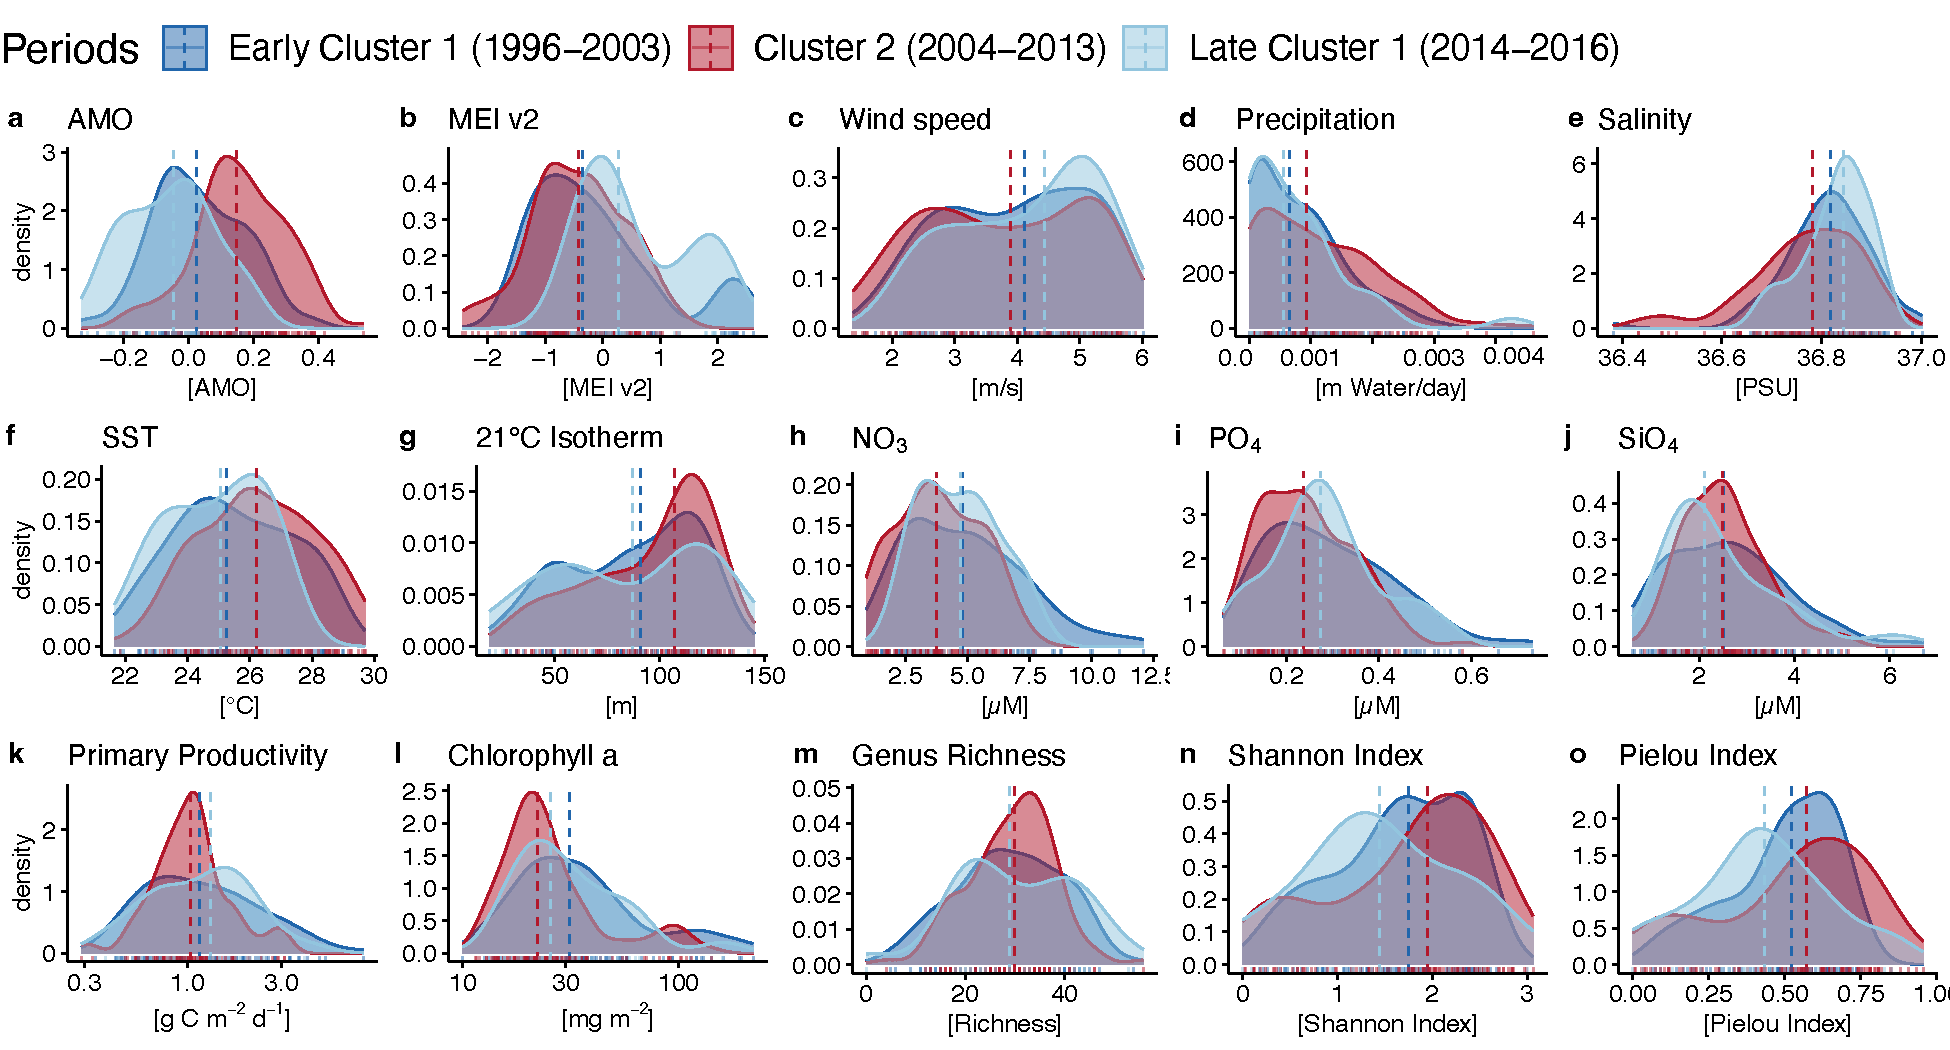
\includegraphics[width=\textwidth]{fig/Figure5_DensityDistributions_v3.pdf}
    \caption{Density distributions of environmental variables, chlorophyll \textit{a}, and diversity indices for the two clusters. The dashed lines mark the median of each distribution.}
    \label{fig:clustcomp}
    \end{figure}


    
    \begin{table}[ht]
    \centering
    \caption{Comparison of environmental and biological variables across three clusters: Early Cluster~1 (1996-2003), Cluster~2 (2004-2013), and Late Cluster~1 (2014-2016). P-values are from two-sided Wilcoxon rank-sum tests on the monthly values. Significance levels indicated by asterisks (p-value: ***\textless0.001, **\textless0.01, *\textless0.05), non-significant results show the p-value. Note that sample sizes for Late Cluster~1 are smaller ($n$ = 21-36), which may limit statistical power for comparisons involving this period. A pattern consistent with recovery to pre-2004 conditions is indicated when E-C1 vs C2 and C2 vs L-C1 show significant differences, while E-C1 vs L-C1 does not.}
    \label{tab:ClustCompWilcox}
    \small
    \begin{tabular}{l rrr ccc}
    \hline
    & \multicolumn{3}{c}{Sample size ($n$)} & \multicolumn{3}{c}{Wilcoxon test} \\
    \cmidrule(lr){2-4} \cmidrule(lr){5-7}
    Variable & E-C1 & C2 & L-C1 & E-C1 vs C2 & C2 vs L-C1 & E-C1 vs L-C1 \\
    \hline
    AMO & 96 & 120 & 36 & *** & *** & ** \\
    MEI v.2 & 96 & 120 & 36 & {\scriptsize 0.38} & *** & *** \\
    Wind speed & 96 & 120 & 36 & {\scriptsize 0.29} & {\scriptsize 0.12} & {\scriptsize 0.43} \\
    Precipitation & 96 & 120 & 36 & * & * & {\scriptsize 0.50} \\
    Salinity & 89 & 111 & 22 & ** & * & {\scriptsize 0.28} \\
    SST & 93 & 111 & 21 & ** & ** & {\scriptsize 0.23} \\
    21°C Isotherm & 93 & 111 & 21 & * & {\scriptsize 0.38} & {\scriptsize 0.87} \\
    NO$_3$ & 84 & 102 & 21 & ** & {\scriptsize 0.07} & {\scriptsize 1.00} \\
    PO$_4$ & 90 & 111 & 21 & * & {\scriptsize 0.16} & {\scriptsize 0.88} \\
    SiO$_4$ & 91 & 110 & 21 & {\scriptsize 0.97} & {\scriptsize 0.28} & {\scriptsize 0.53} \\
    Primary Productivity & 91 & 89 & 22 & {\scriptsize 0.33} & {\scriptsize 0.34} & {\scriptsize 0.96} \\
    Chlorophyll $a$ & 92 & 110 & 22 & *** & {\scriptsize 0.07} & {\scriptsize 0.57} \\
    Diatoms & 87 & 108 & 23 & *** & ** & ** \\
    Haptophytes & 87 & 108 & 23 & *** & *** & {\scriptsize 0.98} \\
    Dinoflagellates & 87 & 108 & 23 & *** & *** & {\scriptsize 0.37} \\
    Cyanobacteria & 87 & 108 & 23 & *** & *** & * \\
    Nanoflagellates & 87 & 108 & 23 & * & *** & *** \\
    Genus Richness & 87 & 108 & 23 & {\scriptsize 0.81} & {\scriptsize 0.71} & {\scriptsize 0.70} \\
    Shannon Index & 87 & 108 & 23 & {\scriptsize 0.17} & {\scriptsize 0.10} & {\scriptsize 0.24} \\
    Pielou Index & 87 & 108 & 23 & {\scriptsize 0.10} & * & {\scriptsize 0.08} \\
    \hline
    \end{tabular}
    \end{table}
    

\subsection{AMO and upwelling-related variables drive community changes}
    % Figure 6
    To identify the variables that best predict the shifts observed within the phytoplankton community, we performed a gradient forest analysis on the monthly microscopy cell counts interpolated over the top 100 meters and grouped by identified genus. Preliminary model runs were made to determine whether time lags of the predictor variables could better explain the data (see Appendix), resulting in the selection of the AMO with a lag of 2 months and MEI v.2 with a lag of 4 months. Figure \ref{fig:GF} $a$ shows the predictor variables ranked by their weighted importance, with the AMO and MEI v.2 indices with time lags, as well as upwelling-related variables such as SST and nitrate in the upper 100 meters, demonstrating the highest predictive capacity. The \qty{21}{\celsius} isotherm, precipitation, and phosphate concentration scored the lowest in predicting changes within the community. 
    Gradient forest predicts shifts in the community by building a random forest model for each observed genus across the time series. The predictive power of the models for each genus is shown in Figure \ref{fig:GF} $b$. The microscopy data are biased toward larger cell sizes and, therefore, most of the predicted genus cell counts are diatoms. However, two haptophyte and three dinoflagellate genera rank relatively high. For the presented run a total of 89 genera (each observed more than 10 times over the time series) were used as indicator variables, of which 46 genera could be predicted using the given predictor variables, which corresponds to more than \qty{95}{\%} of counted cells (see Table \ref{tab:sup:GenusFuncGroups} for a complete list of identified genera). 
    Figure \ref{fig:GF} $c$ shows the cumulative importance of the predictor variables across the parameter range. The dashed black lines indicate cumulative importance across the entire community, and the solid colored lines indicate importance per phytoplankton group. 
    \linelabel{R1:C24:start} Cumulative importance curves from gradient forest analysis show how the importance of a predictor accumulates across its range of values. The slope of the curve at any point indicates where the strongest compositional turnover occurs—steep sections represent threshold values where small changes in the predictor correspond to large changes in community composition, while flat sections indicate regions where the predictor has little influence on community structure. For the AMO index, we see a clear pattern in which negative anomalies affect the community (slope is highest for negative values). \linelabel{R1:C24:end} This contrasts with a higher importance for positive anomalies in the MEI v.2 index, particularly for haptophytes and cyanobacteria. Nitrate concentrations between 6 and 8 \unit{\micro \mole} represent the range within which the community changed most, indicating these values as a threshold for community composition. Figure \ref{fig:sup:GFoutput_lags_extra} in Appendix shows response curves for all variables not shown here. Variables that show a pronounced threshold response are evaporation and salinity. For evaporation the threshold is at larger values of evaporation, which are most likely linked to periods of strong stratification, and salinity at both extreme ends of the range, signifying effects on cell counts of diatoms, dinoflagellates and cyanobacteria at strong upwelling and stratified conditions. 
    
    \begin{figure}
    \noindent\includegraphics[width=\textwidth]{fig/Figure6_NEW_GF_output_LAGGED.pdf}
    \caption{Gradient forest analysis of monthly community data at a genus level. (a) Predictor variables ranked according to overall weighted importance in predicting shifts in abundances. (b) Phytoplankton genera that could be predicted ranked according to the predictive power via the weighted importance. (c) Cumulative importance curves for the predictor variables. The dashed black lines show cumulative importance across predictor range for the entire model and all genera. Solid colored lines represent the responses of individual functional groups.}
    \label{fig:GF}
    \end{figure}
    
    



\section{Discussion}

\subsection{Community reorganization and biomass shifts}
    % P1: Introductory paragraph highlighting the overall dynamics/shifts
    This study shows the long-term dynamics of a tropical coastal marine ecosystem driven by local environmental variability, which is, in turn, influenced by large-scale climatic changes. In the Cariaco Basin, decadal-scale climate oscillations impacted the wind-driven upwelling regime, producing corresponding effects on the composition and biodiversity of the phytoplankton community.
    These changes are clearly visible in the yearly mean anomalies and the density distribution of monthly measurements. After 2004, we observed increased SST, decreased wind speeds, reduced fluorometric chlorophyll \textit{a}, and drastically reduced cell counts of functional groups, all coincident with a shift in the AMO index toward positive mean anomalies until 2014. \linelabel{R2:C26} Comparison of the period following the shift (2005–2013) against the 1996–2004 baseline reveals that average cell counts for diatoms and dinoflagellates were 12.5-fold and 7.2-fold lower, respectively, while cyanobacteria decreased 19.3-fold. Fluorometric chlorophyll a concentrations also decreased, but to a lesser extend (1.6-fold), indicating that the microscopy cell counts overestimate the reduction in phytoplankton biomass.
    By considering the phytoplankton community time series up to the end of 2017, the temporally complete dataset, we found that the observed shift that occurred in 2004 appears to have produced a temporary regime that lasted only until 2014 (cluster 2), when the system shows sign of reverting to a regime similar to that of 1996-2004 (cluster 1), confirming the observations by \citeA{muller-karger_scientific_2019}. In 2014, physical conditions in the Cariaco Basin returned to a regime of increased wind speed, increased upwelling, and elevated nutrient concentrations. Concurrently, we observed an increase in chlorophyll \textit{a} and a return to a community composition more similar to the period between 1996 and 2004. \linelabel{R2:C24}This return to Cluster~1 reflects similarity in overall taxonomic composition, as measured by presence-absence (binary Jaccard distance), rather than in dominant taxa. The identity of dominant genera differed among periods, shifting from \textit{Thalassiosira}/\textit{Pseudo-nitzschia} in 1996-2004, to \textit{Pseudo-nitzschia}/\textit{Emiliania} in 2005-2013, to \textit{Emiliania}/\textit{Thalassiosira} in 2014-2016, yet the clustering analysis indicates that the broader taxonomic pool present in Late Cluster~1 more closely resembled Early Cluster~1 than the intermediate period.
    
    % P2: Discuss community reorganisation, biomass shifts vs HPLC data 
    When comparing the two clusters, we observed a marked reduction in cell counts, which corresponded to a decreased concentration of chlorophyll \textit{a}, particularly in the top \qty{25}{meters} of the water column (see Figure \ref{fig:divts}). The decline in cell counts was not proportional to the more modest decrease in total chlorophyll \textit{a}, suggesting that the phytoplankton community might have transitioned to smaller cells, which were probably below the detection size limit of optical microscopes \cite{muller-karger_scientific_2019}. \linelabel{R2:C28} This shift to smaller cell sizes and a reduction in large diatoms is consistent with predicted effects of warming and reduced mixing on phytoplankton communities \cite{bopp_response_2005}. Increases in temperature can lead to a decrease in the relative contribution of larger cells in the community, irrespective of nutrient availability, but shifts towards smaller cells are particularly prevalent when temperatures increase and nutrient supply decreases \cite{acevedo-trejos_glimpse_2014, mousing_global_2014}, as we observed in the Cariaco Basin. 
    
    % Disucssion of HPLC vs Microscopy!
    Comparison with High-Performance Liquid Chromatography (HPLC) data from the Cariaco Basin \cite{pinckney_phytoplankton_2015} revealed both similarities and differences with our results. While general patterns aligned, the HPLC data showed an increase in chlorophyll \textit{a} between 1996--2000 and 2006--2010, particularly at depths below \qty{55}{\meter}. However, the HPLC data were analyzed by multiple laboratories with a gap in coverage between 2000 and 2006, and total chlorophyll \textit{a} could not be quantified consistently across laboratories \cite{pinckney_phytoplankton_2015}. For this reason, we focused our analysis on the more temporally complete microscopy cell count and fluorometric chlorophyll \textit{a} data. Our results are corroborated by independent spectrophotometric measurements at \qty{20}{\meter} depth off Margarita Island, which similarly showed reduced chlorophyll concentrations between 2004 and 2014 \cite{gomez_gaspar_variacion_2025}.
    Notably, the decline in microscopy cell counts was more pronounced than the decrease in fluorometric chlorophyll \textit{a}, suggesting that the phytoplankton community shifted toward smaller cell sizes below the detection limit of light microscopy. This interpretation is further supported by the HPLC data, which indicated an increase in non-diatom taxa during the 2006--2010 period \cite{pinckney_phytoplankton_2015}.
    \linelabel{R2:C14} The vertical redistribution of chlorophyll is likely linked to changes in euphotic zone depth \citep{lorenzoni_characterization_2015, pinckney_phytoplankton_2015}. Unfortunately, PAR data were not collected during the CARIACO time series and euphotic depth measurements are only available until 2012, precluding direct analysis of light-driven vertical distribution changes across the full study period.

    % P2: Discuss community reorganisation, biomass shifts, and comparison with HPLC data 
    When comparing the two clusters, we observed a marked reduction in cell counts, which corresponded to a decreased concentration of chlorophyll \textit{a}, particularly in the top \qty{25}{\meter} of the water column (Figure \ref{fig:divts}). Notably, the decline in microscopy cell counts was more pronounced than the decrease in fluorometric chlorophyll \textit{a}, suggesting that the phytoplankton community shifted toward smaller cell sizes below the detection limit of light microscopy \cite{muller-karger_scientific_2019}. This shift to smaller cell sizes and a reduction in large diatoms is consistent with predicted effects of warming and reduced mixing on phytoplankton communities \cite{bopp_response_2005}. Such shifts are particularly prevalent when temperatures increase and nutrient supply decreases \cite{acevedo-trejos_glimpse_2014, mousing_global_2014}, as we observed in the Cariaco Basin.
    
    Comparison with High-Performance Liquid Chromatography (HPLC) data from the Cariaco Basin revealed both similarities and differences with our results. While general patterns aligned, the HPLC data showed an increase in chlorophyll \textit{a} between 1996--2000 and 2006--2010, particularly at depths below \qty{55}{\meter} \cite{pinckney_phytoplankton_2015}. However, the HPLC data were analyzed by multiple laboratories with a gap in coverage between 2000 and 2006, and total chlorophyll \textit{a} could not be quantified consistently across laboratories \cite{pinckney_phytoplankton_2015}. For this reason, we focused our analysis on the more temporally complete microscopy cell count and fluorometric chlorophyll \textit{a} data. Our results are corroborated by independent spectrophotometric measurements at \qty{20}{\meter} depth off Margarita Island, which similarly showed reduced chlorophyll concentrations between 2004 and 2014 \cite{gomez_gaspar_variacion_2025}. The shift toward smaller cells is further supported by the HPLC data, which indicated an increase in non-diatom taxa during the 2006-2010 period \cite{pinckney_phytoplankton_2015}.
    
    Our depth-resolved analysis also suggested a a deepening of the chlorophyll maximum during periods of reduced upwelling, in accordance with the findings from HPLC data \cite{pinckney_phytoplankton_2015}. This vertical redistribution is likely linked to changes in euphotic zone depth, documented as 60-75~m during stratified, low-production periods compared to 15-30~m during upwelling \citep{lorenzoni_characterization_2015, pinckney_phytoplankton_2015}. Unfortunately, PAR data were not collected during the CARIACO time series and euphotic depth measurements are only available until 2012, precluding direct analysis of light-driven vertical distribution changes across the full study period.


    
    % P3: Shift in Diversity does not match shift in biomass/cell counts, why?
    The temporal dynamics found in yearly mean genus richness, however, did not correspond directly to the observed clusters. Instead, there was a marked reduction from 1998 to 2009, after which richness recovered four years prior to 2014, when the community returned to levels characteristic of cluster 1. The same trend was evident, albeit to a lesser degree, in the other diversity metrics. Generally, mean annual anomalies in Shannon diversity and Pielou's evenness correlated with genus richness and exhibited a reduced yearly mean between 2000 and 2006, during which cell counts recorded an increase in nanoflagellates and a pronounced peak in cyanobacteria.
    We did not find a significant difference in diversity between the two clusters, either by Shannon index or by genus richness (Figures \ref{fig:zscore} and \ref{fig:divts}). However, we did observe a significant difference in Pielou's index between the two clusters. The results suggest that the phytoplankton community became more evenly distributed during the low upwelling conditions of cluster 2, which is consistent with the analysis of \citeA{pinckney_phytoplankton_2015} based on HPLC pigment data. This increase in evenness, quantified by the Pielou index, is most likely explained by the lack of strong upwelling events and the resulting reduced disturbance of the community. Under strong upwelling conditions, r-selected species are typically favored, leading to dominance by fewer taxa and consequently lower evenness. A decrease in compositional turnover was also observed in a decline in interannual species turnover during cluster 2 (see Figure \ref{fig:clustering} $b$). As the productivity and biomass of phytoplankton communities are driven primarily by nutrients supplied through disturbance events, this is in line with the inverse relationship between evenness and community performance observed in previous studies \cite{lehtinen_phytoplankton_2017, otero_phytoplankton_2020}.
    
    

\subsection{Drivers of change}
    % P4: Introduce GF Analysis and discuss results
    To identify the variables that best predict changes in the phytoplankton community, we conducted a gradient forest analysis using time series of climate indices and in situ measurements to predict genus-level abundances from microscopy cell counts. Gradient forest is an extension of the random forest algorithm, designed to identify thresholds and patterns in community composition along environmental gradients \cite{ellis_gradient_2012}. Limiting the analysis to bottom-up drivers ensured the greatest possible data coverage throughout the CARIACO time series. Interestingly, our analysis revealed that the strongest predictor of change within the community was not an in situ measurement but rather the AMO index. The AMO index is followed in importance by SST, the MEI v.2, and nitrate concentration as predictive variables (see Figure \ref{fig:GF}).
    
    % P5: Climate impacts
    Although regional effects may vary, a negative phase in the AMO is generally associated with periods of colder surface temperatures and a southward shift of the ITCZ \cite{knight_climate_2006, colna2017latitudinal}. In the Cariaco Basin, a southward shift of the ITCZ correlates with increased wind-driven upwelling \cite{taylor_ecosystem_2012}. The threshold responses between functional groups, which relate to shifts in cell count abundances, showed contrasting patterns. Diatoms, dinoflagellates, and haptophytes exhibited strong response thresholds for negative AMO anomalies, which pointed to the influence of stronger upwelling conditions. The abundance of haptophytes, additionally, showed a threshold effect at positive AMO anomalies, which may be related to the pattern observed by \citeA{pinckney_phytoplankton_2015} based on HPLC data showing haptophytes blooming more frequently during the time period of 2006 to 2010, which was characterized by mostly positive AMO anomalies.
    
    The El Niño Southern Oscillation (ENSO) exhibits a strong teleconnection to the Caribbean Sea. During El Niño (indicated by a positive MEI v.2 index) sea surface temperatures rise, and trade winds blow more to the north-northwest \cite{enfield_tropical_1997}. This would imply a general reduction in upwelling strength during El Niño events in the Cariaco Basin, which has indeed been observed during the period from 1997 to 1998 \cite{romero_seasonal_2009}. The MEI v.2 is significantly positively correlated to local evaporation and salinity and negatively correlated to the AMO index, however it is not significantly correlated to local upwelling-related variables (see Figure \ref{fig:sup:correlation} in Appendix). The link here is less clear; while generally trade wind strength and SST are anti-correlated in the Caribbean Sea, positive trade wind anomalies have been observed during during El Niño conditions and the reverse during La Niña \cite{chang_coupled_2013}. \citeA{taylor_ecosystem_2012} found no strong correlation between MEI v.2 and other variables in the Cariaco Basin, and only \qtyrange{24}{36}{\%} explanation of variance using linear regression with a time lag of 12 months. In contrast, we found a relatively strong predictive power for changes in the phytoplankton community for the MEI v.2 index with a 4-month time lag. We also tested a 12-month time lag and found no significant improvement (Table \ref{tab:sup:GFlagtests} in Appendix).
    The threshold responses indicate a shift in the abundances of dinoflagellates for negative MEI v.2 anomalies, which represent La Niña conditions. Findings from Bayesian modeling showed that dinoflagellates responded positively to warmer, stratified conditions in the Cariaco Basin \cite{mutshinda_environmental_2013}. For cyanobacteria and haptophytes, we observed a pronounced threshold response to positive anomalies, demonstrating sensitivity to ENSO events. Diatoms do not exhibit a clear threshold response, but show a slightly stronger response in the positive range of the MEI v.2. Interestingly, positive anomalies in the MEI v.2, representing strong ENSO events, are mostly found in the high upwelling regime of cluster 1 (see Figure \ref{fig:clustering} $e$). This could be explained by previous findings, that strong El Niño events (as indicated by a positive MEI) increase the strength of currents in the Caribbean sea through modulating the easterly wind anomalies, thereby potentially increasing upwelling strength in the Cariaco Basin \cite{huang_enso_2023}.
    In particular, this intensification of the Caribbean Current may enhance the secondary upwelling that typically occurs between June and August \cite{rueda-roa_description_2018}, rather than affecting the primary wind-driven upwelling between December and May. Additionally, enhanced eddy activity near the Cariaco Basin during strong El Niño events can stimulate productivity and alter community composition through ventilation of sub-oxic waters below the sill \cite{astor_seasonal_2003}.
    
    The in-situ measurements that best predicted changes in the microphytoplankton community were SST, nitrate concentration, and salinity, in that order. Haptophytes and diatoms exhibited a steep threshold around \qtyrange{22}{24}{\celsius}, indicating the strong effect on cell counts at low surface temperatures that are indicative of strong upwelling. Nitrate is a crucial nutrient for phytoplankton growth and has been identified as the growth-limiting nutrient during stratification periods in the Cariaco Basin \cite{muller-karger_scientific_2019}. For diatoms, a strong threshold response was observed above \qty{7}{\micro M}, indicating that intense upwelling conditions drove growth in large diatoms, resulting in predictable changes in cell counts.
    
    These results matched the observed NMDS clustering of the monthly cell counts in relation to the predictor variables, as the scaling axis that separated the two clusters was NMDS 1, which co-varied most strongly with changes in AMO, MEI v.2, salinity, evaporation, and precipitation (Figure \ref{fig:clustering} $c$). Variables directly related to upwelling conditions, such as temperature, \qty{21}{\celsius} isotherm, wind speed, and nutrient concentrations varied more strongly along NMDS 2. Salinity and silicate concentration, which are also strongly related to water mass exchanges through upwelling but additionally depend on freshwater input from precipitation and surface runoff, showed greater variance along NMDS 1. The fact that salinity and the MEI v.2 align is consistent with the influence of ENSO on regional hydrology, as El Niño events typically result in reduced precipitation and drier conditions in the southern Caribbean, whereas La Niña years are associated with higher precipitation, leading to elevated silicate concentrations and lower surface salinity \cite{giannini_interdecadal_2001}. Salinity, evaporation, and silicate concentration exhibited some explanatory power in the gradient forest analysis, although they were weaker predictors than SST, nitrate concentration, and climate indices (see Figure \ref{fig:GF}). This implies that the climate indices explain variability that more direct measurements of upwelling intensity do not capture. 
    

\subsection{Limitations}
    % P6: Discuss limitations of study and methodology

    % 0. Discussion of missing data and temporal aggregation
    \linelabel{R2:missing-discussion} Our analyses employed different temporal aggregations depending on the research question. Annual aggregation for z-scores and hierarchical clustering was chosen to emphasize interannual trends and reduce the influence of seasonal variability and extreme monthly values on long-term pattern detection. However, annual averaging may mask important sub-annual dynamics, particularly given the strong seasonality of the Cariaco upwelling system. To address this, we complemented annually aggregated analyses with monthly-resolution approaches (NMDS ordination, gradient forest analysis) that preserve seasonal signals.
    %MORE ON MISSING DATA

    % 1.  Discuss Limitations of Light microscopy cell counts in CARIACO Time Series
    \linelabel{R2:C31} Using microscopy cell counts as a basis for our analysis allowed us to focus on changes in the microphytoplankton community. Our choice of grouping cell counts by genus was based on the assumption that species within a genus generally exhibit similar eco-physiological responses. The output of the gradient forest model was further grouped by broad functional types to facilitate the identification of broader ecological shifts and trends. The phytoplankton genera that could be best predicted were mostly diatoms, along with some haptophytes, dinoflagellates, and cyanobacteria (Figure \ref{fig:GF} $b$). This does not represent a complete picture of the phytoplankton community of the Cariaco basin. The HPLC pigment data used by \citeA{pinckney_phytoplankton_2015} captured all size classes of phytoplankton and showed less drastic declines in almost all functional groups after 2004. With the caveat that the microscopy counts captured microphytoplankton almost exclusively, this discrepancy with the HPLC pigment analysis can be explained. Drastic declines in cell counts reflected shifts to smaller species, an aspect consistent with size spectra calculated by previous studies using HPLC pigment data \cite{lorenzoni_characterization_2015}. \linelabel{R2:C8:2} Comparative studies have shown that microscopic estimates become less consistent when small cells dominate the community, and that diatom contributions to total biomass tend to be higher when estimated by microscopy compared to pigment-based methods \citep{schluter2000use, havskum2004routine}. Such different dynamics would clearly also impact the interpretation of environmental effects on the community.
    However, the HPLC dataset had limited temporal coverage and was assembled from four different laboratories, introducing potential inconsistencies. We therefore focused on the microscopy data, which provided continuous genus and species-level observations across the full time series, while acknowledging that our analysis may over- or underestimate the magnitude of community change when shifts occur towards or among smaller size fractions.
    
    % 2. Discuss limitations of GF analysis & Limitation to bottom-up drivers and climate indices
    The limited scope of the microscopy cell counts also affected the conclusions that could be drawn from the gradient forest analysis, as these results are limited to microphytoplankton. 
    Another potential caveat of our methodology is that many of the predictors in ecological time series in general and, specifically, in this study, are correlated (Figure \ref{fig:sup:correlation} in Appendix). This can lead to the identification of a correlated predictor that has no direct effect on community changes. However, the gradient forest methodology addresses this by conditionally permuting subsets of the correlated predictors, which can partly mitigate this problem \cite{ellis_gradient_2012}. Additionally, random forest models do not consider temporal relationships between data points, which is why we included tests for the predictive relationships with time lags of our predictors. Without adjusting for time lags, SST and nitrate concentration are the strongest predictors of community change (Figure \ref{fig:sup:GFoutput_nolags} in Appendix). Incorporating time lags slightly improves the overall predictive strength, as quantified by the $R^2$ weighted importance, although both SST and the AMO index yielded a relatively low value around \qty{0.03}{}. This is expected given the noisy nature of phytoplankton microscopy cell counts and is consistent with values reported in other studies utilizing the gradient forest algorithm \cite{pitcher_exploring_2012, roubeix_identification_2016, samhouri_defining_2017, fraker_temporal_2022}. It is important to consider that although predictive relationships between drivers and ecological variables are identified, this does not necessarily imply a mechanistic causal relationship. The scope of our analysis, like any statistical analysis, is exploratory and aims at narrowing down potential key relationships. Mathematical modeling and experimental work are required to develop a clearer mechanistic understanding of the drivers of ecosystem change in the Cariaco Basin.
     
    Our focus on bottom-up drivers of community change may have restricted the explanatory power of our analysis, as top-down processes such as zooplankton grazing may have impacted the structure of the phytoplankton community \cite{frank_ups_2007, banas_adding_2011, acevedo-trejos_mechanisms_2015}. For instance, a trophic cascade resulting from the collapse of sardine fisheries and a subsequent increase in mesozooplankton abundance was proposed to have affected the phytoplankton community in the Cariaco Basin \cite{rueda-roa_spatial_2017, muller-karger_scientific_2019}. However, this predictor could not be included in our gradient forest analysis due to a lack of data at monthly resolution. Given the scarcity of data covering higher trophic levels and the absence of zooplankton data for the first six years of the time series, we suggest that mechanistic modeling would be the ideal approach for investigating the relative impacts of top-down and bottom-up drivers.
    
    

\section{Conclusions}
    We found that decadal-scale climate variability, particularly linked to the AMO index, strongly influenced phytoplankton community composition in the tropical coastal ecosystem of the Cariaco Basin. Phytoplankton cell counts revealed two distinct community clusters: the first, observed during the early part of the time series (1996–2004), was associated with strong upwelling conditions and negative AMO anomalies. A shift to the second cluster occurred after 2004, characterized by weak upwelling and positive AMO anomalies. While overall diversity remained similar between clusters, the low-upwelling period showed reduced taxonomic turnover and increased evenness. These shifts did not reflect a permanent regime change. Rather, in 2014 the community appears to have returned to a composition resembling the early period, coinciding with indications of a reversion to stronger upwelling conditions and negative AMO anomalies. This return occurred despite ongoing multi-year trends of surface warming, declining productivity, and steep reductions in microphytoplankton abundance, suggesting a degree of resilience in the phytoplankton community to climate-driven perturbations.

    Our findings point to an oscillatory pattern in community structure, with transitions linked to low-frequency climate variability. This highlights the importance of long-term ecological time series for capturing non-linear ecosystem responses and underscores the potential of the AMO as a useful indicator of ecosystem state in this region, in line with the observations of \citeA{nye_ecosystem_2014}. Although our study is subject to some limitations, it provides evidence of a partial return to earlier ecosystem conditions and supports the notion that the phytoplankton community in the Cariaco Basin is shaped by recurring climate cycles. Future work, particularly using mathematical modeling, could help disentangle the relative impact of bottom-up versus top-down drivers, factors that remain largely unexplored in the Cariaco Basin.
 

%%

%  Numbered lines in equations:
%  To add line numbers to lines in equations,
%  \begin{linenomath*}
%  \begin{equation}
%  \end{equation}
%  \end{linenomath*}



%% Enter Figures and Tables near as possible to where they are first mentioned:
%
% DO NOT USE \psfrag or \subfigure commands.
%
% Figure captions go below the figure.
% Acronyms used in figure captions will be spelled out in the final, published version.

% Table titles go above tables;  other caption information
%  should be placed in last line of the table, using
% \multicolumn2l{$^a$ This is a table note.}
% NOTE that there is no difference between table caption and table heading in the final, published version
%
%----------------
% EXAMPLE FIGURES
%
% \begin{figure}
% \includegraphics{example.png}
% \caption{caption}
% \end{figure}
%
% Giving latex a width will help it to scale the figure properly. A simple trick is to use \textwidth. Try this if large figures run off the side of the page.
% \begin{figure}
% \noindent\includegraphics[width=\textwidth]{anothersample.png}
%\caption{caption}
%\label{pngfiguresample}
%\end{figure}
%
%
% If you get an error about an unknown bounding box, try specifying the width and height of the figure with the natwidth and natheight options. This is common when trying to add a PDF figure without pdflatex.
% \begin{figure}
% \noindent\includegraphics[natwidth=800px,natheight=600px]{samplefigure.pdf}
%\caption{caption}
%\label{pdffiguresample}
%\end{figure}
%
%
% PDFLatex does not seem to be able to process EPS figures. You may want to try the epstopdf package.
%

%
% ---------------
% EXAMPLE TABLE
%
% \begin{table}
% \caption{Time of the Transition Between Phase 1 and Phase 2$^{a}$}
% \centering
% \begin{tabular}{l c}
% \hline
%  Run  & Time (min)  \\
% \hline
%   $l1$  & 260   \\
%   $l2$  & 300   \\
%   $l3$  & 340   \\
%   $h1$  & 270   \\
%   $h2$  & 250   \\
%   $h3$  & 380   \\
%   $r1$  & 370   \\
%   $r2$  & 390   \\
% \hline
% \multicolumn{2}{l}{$^{a}$Footnote text here.}
% \end{tabular}
% \end{table}

%%%%%%%%%%%%%%%%%%%%%%%%%%%%%%%%%%%%%%%%%%%%%%%
% SIDEWAYS FIGURES and TABLES
% AGU prefers the use of {sidewaystable} over {landscapetable} as it causes fewer problems.
%
% \begin{sidewaysfigure}
% \includegraphics[width=20pc]{figsamp}
% \caption{caption here}
% \label{newfig}
% \end{sidewaysfigure}
%
%  \begin{sidewaystable}
%  \caption{Caption here}
% \label{tab:signif_gap_clos}
%  \begin{tabular}{ccc}
% one&two&three\\
% four&five&six
%  \end{tabular}
%  \end{sidewaystable}

%% If using numbered lines, please surround equations with \begin{linenomath*}...\end{linenomath*}
%\begin{linenomath*}
%\begin{equation}
%y|{f} \sim g(m, \sigma),
%\end{equation}
%\end{linenomath*}

%%% End of body of article

%%%%%%%%%%%%%%%%%%%%%%%%%%%%%%%%%%%%%%%%%%%%%%%
%% Optional Appendices go here
%
% The \appendix command resets counters and redefines section heads
%
% After typing \appendix
%
%\section{Here Is Appendix Title}
% will show
% A: Here Is Appendix Title
%

\appendix
\newpage
\section{Correlation of data}

\begin{figure}[h!]
\noindent\includegraphics[width=\textwidth]{fig/CorrClustSupplementalPlot_v2.pdf}
\caption{Correlation matrix with clustering of environmental variables, diversity metrics and cell counts. Biological variables (chlorophyll \textit{a}, primary productivity, and phytoplankton group abundances) were log-transformed (log\textsubscript{1+x}) prior to analysis. Correlation was calculated using Spearman's rank correlation coefficient; the magnitude of the coefficient is indicated by the color of the circle. The size of the circle and significance level marking represents the calculated significance of the correlation deviating from 0 (p-value: ***\textless0.001, **\textless0.01, *\textless0.05). The time series were additionally ordered by hierarchical clustering via the complete linkage method into 5 groups indicated by the black square border. Note that significance levels should be interpreted with caution, as temporal autocorrelation in the monthly time series may inflate the apparent statistical significance of correlations.}
\label{fig:sup:correlation}
\end{figure}



\newpage
\section{Gradient forest analysis supplement}


\begin{figure}[h!]
\noindent\includegraphics[width=\textwidth]{fig/Figure6_NEW_GF_supplement_LAGGED.pdf}
\caption{Cumulative importance curves for all predictor variables not shown in the main figure. Dashed black line represents the cumulative importance across the entire community, colored lines represent functional groups. Gradient forest runs where done on Genus-level cell counts, integrated over the top 100 meters.}
\label{fig:sup:GFoutput_lags_extra}
\end{figure}


\begin{table}
\centering
\caption{\label{tab:tab:sup:GFlagtests}Resulting $R^2$ weighted importance for running predictor variables together with time-lags to check if they provide a better fit to the data. Each column represents a single run, with resulting importance values for time series and monthly lags. The results were stable, so that repeated runs confirmed the chosen time lag. For in-situ variables, we tested all measurements up to a lag of 3 months. For climate variables we tested up to a lag of 12 months and lags of 1 to 5 years (i.e. 12 - 60 months). Time lag with maximum importance per variable are highlighted in bold and chosen for the final model run.}
\centering
\resizebox{\ifdim\width>\linewidth\linewidth\else\width\fi}{!}{
\begin{tabular}[t]{rllllllllll}
\toprule
lag (months)& NO3 & PO4 & SiO4 & SST & \qty{21}{\celsius} Isotherm & Salinity & Wind speed & Precipitation & AMO & MEI v.2\\
\midrule
0 & \textbf{0.062} & \textbf{0.029} & \textbf{0.022} & \textbf{0.1} & \textbf{0.037} & 0.007 & 0.003 & 0.004 & 0.006 & 0.006\\
1 & 0.027 & 0.013 & 0.014 & 0.007 & 0.012 & 0.005 & \textbf{0.009} & \textbf{0.011} & 0.005 & 0.004\\
2 & 0.019 & 0.007 & 0.01 & 0.006 & 0.007 & \textbf{0.014} & 0.007 & 0.004 & 0.005 & 0.003\\
3 & 0.013 & 0.008 & 0.008 & 0.009 & 0.005 & 0.008 & 0.005 & 0.008 & 0.006 & 0.003\\
4 & NA & NA & NA & NA & NA & NA & 0.006 & 0.008 & 0.005 & 0.004\\

5 & NA & NA & NA & NA & NA & NA & 0.008 & 0.008 & 0.002 & 0.004\\
6 & NA & NA & NA & NA & NA & NA & 0.006 & 0.007 & 0.003 & 0.004\\
7 & NA & NA & NA & NA & NA & NA & NA & NA & 0.002 & 0.004\\
8 & NA & NA & NA & NA & NA & NA & NA & NA & 0.003 & 0.004\\
9 & NA & NA & NA & NA & NA & NA & NA & NA & 0.002 & 0.004\\

10 & NA & NA & NA & NA & NA & NA & NA & NA & 0.003 & 0.003\\
11 & NA & NA & NA & NA & NA & NA & NA & NA & 0.003 & 0.005\\
12 & NA & NA & NA & NA & NA & NA & NA & NA & 0.005 & 0.007\\
\addlinespace
24 & NA & NA & NA & NA & NA & NA & NA & NA & \textbf{0.031} & 0.02\\
36 & NA & NA & NA & NA & NA & NA & NA & NA & 0.023 & 0.018\\
48 & NA & NA & NA & NA & NA & NA & NA & NA & 0.016 & \textbf{0.03}\\
60 & NA & NA & NA & NA & NA & NA & NA & NA & 0.02 & 0.025\\
\bottomrule
\end{tabular}}

\label{tab:sup:GFlagtests}
\end{table}


\begin{figure}
\noindent\includegraphics[width=\textwidth]{fig/Figure6_NEW_GF_output_NOLAG.pdf}
\caption{Gradient forest analysis of monthly community data at a genus level for all predictors without any time lags. (a) Predictor variables ranked according to overall weighted importance in predicting shifts in abundances. (b) Phytoplankton genera that could be predicted ranked according to the predictive power via the weighted importance. (c) Cumulative importance curves for the predictor variables. The dashed black lines show cumulative importance across predictor range for the entire model and all genera. Solid colored lines represent the responses of individual functional groups.}
\label{fig:sup:GFoutput_nolags}
\end{figure}


\begin{figure}
\noindent\includegraphics[width=\textwidth]{fig/Figure6_NEW_GF_supplement_NOLAG.pdf}
\caption{Cumulative importance curves for all variables not shown in the previous figure, showing the gradient forest analysis performed with all predictors without any time lags. Dashed black line represents the cumulative importance across the entire community. Solid colored lines represent functional groups. Gradient forest runs where done on Genus-level cell counts, integrated over the top 100 meters.}
\label{fig:sup:GFoutput_nolags_extra}
\end{figure}



%\end{tabular}}

%\label{tab:sup:GenusFuncGroups}
%\end{table}

%\begin{table}

%\caption{Table \ref{tab:sup:GenusFuncGroups} cont.:}
%\begin{tabular}{@{}ll@{}}

%
\begin{table}
\caption{Table of all identified genus that were counted more than 10 times across the time series (n=89). The monthly cell counts per genus were used as input data to the gradient forest analysis.}
% Please add the following required packages to your document preamble:
% \usepackage{booktabs}

%\resizebox*{\textheight}{!}{
\resizebox*{!}{\dimexpr\textheight-\lineskip\relax}{%
\begin{tabular}{@{}ll@{}}
\textbf{Diatoms} &                                                            \\
\textit{Amphora}           & C.G. Ehrenberg ex F.T. Kützing, 1844                       \\
\textit{Asterionella}      & A.H. Hassall, 1850                                         \\
\textit{Asterionellopsis}  & F.E. Round in F.E. Round, R.M. Crawford \& D.G. Mann, 1990 \\
\textit{Bacteriastrum}     & G. Shadbolt, 1854                                          \\
\textit{Bellerochea}       & H. Van Heurck, 1885                                        \\
\textit{Cerataulina}       & H. Peragallo ex F. Schütt in Engler \& Prantl, 1896        \\
\textit{Chaetoceros}       & C.G. Ehrenberg, 1844                                       \\
\textit{Climacodium}       & A. Grunow, 1868                                            \\
\textit{Corethron}         & A.F. Castracane, 1886                                      \\
\textit{Coscinodiscus}     & C.G. Ehrenberg, 1839                                       \\
\textit{Cylindrotheca}     & L. Rabenhorst, 1859                                        \\
\textit{Dactyliosolen}     & A.F. Castracane, 1886                                      \\
\textit{Detonula}          & F. Schütt ex G.B. De Toni, 1894                            \\
\textit{Diploneis}         & (C. G. Ehrenberg) P.T. Cleve, 1894                         \\
\textit{Eucampia}          & C.G. Ehrenberg, 1839                                       \\
\textit{Grammatophora}     & C.G. Ehrenberg, 1840                                       \\
\textit{Guinardia}         & H. Peragallo, 1892                                         \\
\textit{Haslea}            & R. Simonsen, 1974                                          \\
\textit{Helicotheca}       & M. Ricard, 1987                                            \\
\textit{Hemiaulus}         & P.A.C. Heiberg, 1863                                       \\
\textit{Lauderia}          & P.T. Cleve, 1873                                           \\
\textit{Leptocylindrus}    & P.T. Cleve in C.G.J. Petersen, 1889                        \\
\textit{Lioloma}           & Hasle, 1997                                                \\
\textit{Navicula}          & J.B.M. Bory de Saint-Vincent, 1822                         \\
\textit{Nitzschia}         & A.H. Hassall, 1845                                         \\
\textit{Odontella}         & C.A. Agardh, 1832                                          \\
\textit{Pinnularia}        & C.G. Ehrenberg, 1843                                       \\
\textit{Pinnunavis}        & H. Okuno, 1975                                             \\
\textit{Planktoniella}     & (C.G.Wallich) Schütt, 1892                                 \\
\textit{Pleurosigma}       & W. Smith, 1852                                             \\
\textit{Proboscia}         & G. Sundström, 1986                                         \\
\textit{Pseudo-nitzschia}  & H. Peragallo in H. Peragallo \& M. Peragallo, 1900         \\
\textit{Rhizosolenia}      & T. Brightwell, 1858                                        \\
\textit{Skeletonema}       & R.K. Greville, 1865                                        \\
\textit{Sundstroemia}      & Medlin, Boonprakob, Lundholm \& Moestrup, 2021             \\
\textit{Tabularia}         & (F.T. Kutzing) D.M. Williams \& F.E. Round, 1986           \\
\textit{Thalassionema}     & A. Grunow ex C. Mereschkowsky, 1902                        \\
\textit{Thalassiosira}     & P.T. Cleve, 1873 emend. Hasle, 1973                        \\
\textbf{Cyanobacteria}     &                                                            \\
\textit{Anabaena}          & Bory de Saint-Vincent ex Bornet \& Flahault, 1886          \\
\textit{Johannesbaptistia} & G.De Toni, 1934                                            \\
\textit{Lyngbya}           & C.Agardh ex Gomont, 1892                                   \\
\textit{Synechococcus}     & Nägeli, 1849                                               \\
\textit{Trichodesmium}     & Ehrenberg ex Gomont, 1892                                  \\
\textbf{Dinoflagellates}    &                                                            \\
\textit{Akashiwo}          & Gert Hansen \& Moestrup, 2000                              \\
\textit{Alexandrium}       & Halim, 1960                                                \\
\textit{Amphidinium}       & Claperède \& Lachmann, 1859                                \\
\textit{Blepharocysta}     & Ehrenberg, 1873                                            \\
\textit{Cochlodinium}      & Schütt, 1896                                               \\
\textit{Cystodinium}       & Klebs, 1912                                                \\

\textit{Dinophysis}        & Ehrenberg, 1839                                            \\
\textit{Diplopsalis}       & R.S.Bergh, 1881                                            \\
\textit{Glenodinium}       & Ehrenberg, 1836     
\\
\textit{Gonyaulax}         & Diesing, 1866                                              \\
\textit{Gymnodinium}       & F.Stein, 1878                                              \\
\textit{Gyrodinium}        & Kofoid \& Swezy, 1921                                      \\
\textit{Heterocapsa}       & F.Stein, 1883                                              \\
\textit{Lingulodinium}     & D.Wall, 1967                                               \\
\textit{Mesoporos}         & Lillick, 1937                                              \\
\textit{Ornithocercus}     & Stein, 1883                                                \\
\textit{Oxytoxum}          & Stein, 1883                                                \\
\textit{Phalacroma}        & Stein, 1883                                                \\
\textit{Oxyphysis}         & Kofoid, 1926                                               \\
\textit{Podolampas}        & F.Stein, 1883                                              \\
\textit{Pronoctiluca}      & Fabre-Domergue, 1889                                       \\
\textit{Prorocentrum}      & Ehrenberg, 1834                                            \\
\textit{Exuviella}         & Cienkowski, 1881                                           \\
\textit{Protoperidinium}   & Bergh, 1881                                                \\
\textit{Pyrocystis}        & J.Murray ex Haeckel, 1890                                  \\
\textit{Pyrophacus}        & F.Stein, 1883                                              \\
\textit{Scrippsiella}      & Balech ex A.R.Loeblich III, 1965                           \\
\textit{Sphaerodinium}     & Woloszynska, 1916                                          \\
\textit{Triadinium}        & Dodge, 1981                                                \\
\textit{Tripos}            & Bory de Saint-Vincent, 1823                                \\
\textbf{Haptophytes}        &                                                            \\
\textit{Calcidiscus}       & Kamptner, 1950                                             \\
\textit{Calciopappus}      & Gaarder \& Ramsfjell, 1954                                 \\
\textit{Calciosolenia}     & Gran, 1912                                                 \\
\textit{Calyptrosphaera}   & Lohmann, 1902                                              \\
\textit{Coccolithus}       & E.H.L.Schwarz, 1894                                        \\
\textit{Cyclolithella}     & Loeblich \& Tappan, 1963                                   \\
\textit{Emiliania}         & W.W.Hay \& H.P.Mohler, 1967                                \\
\textit{Michaelsarsia}     & Gran, 1912                                                 \\
\textit{Ophiaster}         & Gran, 1912                                                 \\
\textit{Syracosphaera}     & Lohmann, 1902                                              \\
\textit{Umbellosphaera}    & Paasche, 1955                                              \\
\textit{Umbilicosphaera}   & Lohmann, 1902                                              \\
\textbf{Others}            &                                                            \\
\textit{Dictyocha}         & Ehrenberg, 1837                                            \\
\textit{Eutreptia}         & Perty, 1852                                                \\
\textit{Eutreptiella}      & A.M.Cunha, 1913                                            \\
\textit{Mesodinium}        & von Stein                                                 
\end{tabular}}

\label{tab:sup:GenusFuncGroups}
\end{table}



\newpage
\section{Seasonal effect supplemental information}

\begin{figure}[h]
\centering
\noindent\includegraphics[width=300px]{fig/FigureSX_seasonalNMDS_v1.pdf}
\caption{NMDS plot of monthly phytoplankton community data (genus-level cell counts, cube-root transformed) with points colored by season. Stress: 0.263, 2 dimensions, converging solution. Vectors show how environmental variables co-vary with the community data; vector length indicates the strength of the relationship. No clear separation is visible among seasonal groups (Upwelling: December-May; Secondary Upwelling: June-August; Rainy: September-November), consistent with PERMANOVA results showing that season explains only 3.5\% of community variance compared to 17.9\% for interannual cluster (Table~\ref{tab:sup:permanova_season_cluster}).}
\label{fig:sup:nmds_season}
\end{figure}

\begin{table}[h]
\centering
\caption{Permutational multivariate analysis of variance (PERMANOVA) testing the effects of interannual cluster and season on phytoplankton community composition. Community data (genus-level cell counts) were cube-root transformed prior to analysis. Bray-Curtis dissimilarity was used as the distance metric, with 999 permutations. Two observations (1995, 2017) were excluded due to missing cluster assignments ($n$ = 193). Results shown are for cluster entered first; reversing term order yielded nearly identical R\textsuperscript{2} values (cluster: 17.9\%, season: 3.5\%), indicating minimal collinearity between factors.}
\label{tab:sup:permanova_season_cluster}
\small
\begin{tabular}{l rrrrl}
\hline
Factor & df & Sum of Squares & R\textsuperscript{2} (\%) & \textit{F} & \textit{p}-value \\
\hline
Cluster & 2 & 8.772 & 17.9 & 21.4 & 0.001 \\
Season & 2 & 1.713 & 3.5 & 4.2 & 0.001 \\
Residual & 188 & 38.525 & 78.6 & — & — \\
Total & 192 & 49.010 & 100.0 & — & — \\
\hline
\end{tabular}
\end{table}


\begin{table}
\centering
\caption{\label{tab:sup:GFlagtests_seasonal}Mean $R^2$ weighted importance for predictor variables across three seasons, used to select optimal time lags. Values shown as: lag in months (mean importance). Due to relatively small seasonal sample sizes and resulting stochasticity in importance estimates, the analysis was run five times per season and mean values are reported. For in-situ variables, lags of 0-3 months were tested; for atmospheric variables, 0-6 months; for climate indices, 0-12, 24, 36, 48, and 60 months. To balance model parsimony with explanatory power, the shortest lag within 20\% of maximum importance was selected (bold), favoring more directly interpretable ecological relationships when predictive performance was similar.}
\centering
\resizebox{\ifdim\width>\linewidth\linewidth\else\width\fi}{!}{
\begin{tabular}[t]{llll}
\toprule
Variable & Upwelling & Secondary Upwelling & Rainy\\
\midrule
\addlinespace[0.3em]
\multicolumn{4}{l}{In-situ variables (lags 0-3 months)}\\
\hspace{1em}NO\textsubscript{3} & \textbf{0} (0.060); 1 (0.036); 2 (0.020) & \textbf{0} (0.034); 3 (0.031); 2 (0.029) & 3 (0.017); \textbf{0} (0.015); 2 (0.006)\\
\hspace{1em}PO\textsubscript{4} & \textbf{0} (0.023); 1 (0.008); 2 (0.007) & 3 (0.023); \textbf{0} (0.021); 2 (0.020) & \textbf{0} (0.039); 3 (0.027); 1 (0.014)\\
\hspace{1em}SiO\textsubscript{4} & \textbf{0} (0.026); 1 (0.008); 3 (0.006) & \textbf{0} (0.032); 1 (0.028); 2 (0.022) & \textbf{3} (0.043); 1 (0.033); 2 (0.032)\\
\hspace{1em}SST & \textbf{0} (0.101); 3 (0.014); 1 (0.007) & \textbf{0} (0.032); 2 (0.025); 1 (0.014) & \textbf{0} (0.052); 1 (0.032); 3 (0.010)\\
\hspace{1em}\qty{21}{\celsius} Isotherm & \textbf{0} (0.045); 1 (0.011); 2 (0.007) & \textbf{1} (0.024); 3 (0.014); 0 (0.010) & \textbf{0} (0.032); 2 (0.010); 3 (0.007)\\
\hspace{1em}Salinity & \textbf{0} (0.031); 3 (0.010); 2 (0.008) & \textbf{2} (0.073); 3 (0.049); 1 (0.020) & \textbf{0} (0.022); 3 (0.010); 2 (0.010)\\
\addlinespace[0.3em]
\multicolumn{4}{l}{Atmospheric variables (lags 0-6 months)}\\
\hspace{1em}Wind speed & 5 (0.007); 6 (0.007); 4 (0.006) & \textbf{6} (0.027); 2 (0.010); 5 (0.006) & \textbf{0} (0.021); 5 (0.019); 2 (0.009)\\
\hspace{1em}Precipitation & \textbf{1} (0.019); 0 (0.012); 2 (0.009) & \textbf{0} (0.018); 2 (0.012); 1 (0.008) & \textbf{3} (0.017); 0 (0.012); 6 (0.006)\\
\addlinespace[0.3em]
\multicolumn{4}{l}{\textit{Climate indices (lags 0-12, 24, 36, 48, 60 months)}}\\
\hspace{1em}AMO & 60 (0.028); \textbf{24} (0.023); 36 (0.021) & \textbf{24} (0.034); 60 (0.032); 36 (0.020) & 48 (0.028); \textbf{36} (0.025); 12 (0.013)\\
\hspace{1em}MEI v.2 & \textbf{48} (0.036); 36 (0.018); 60 (0.018) & \textbf{60} (0.037); 24 (0.018); 0 (0.015) & 48 (0.027); \textbf{36} (0.024); 60 (0.020)\\
\bottomrule
\end{tabular}}
\end{table}

\begin{figure}
    \noindent\includegraphics[width=\textwidth]{fig/Figure_GF_seasonal_importance.pdf}
    \caption{Gradient forest analysis of monthly phytoplankton community data at genus level across three oceanographic seasons: (a) Upwelling, (b) Secondary Upwelling, and (c) Rainy. For each season, predictor variables are ranked by $R^2$ weighted importance for models without time lags (left) and with optimal lags (center), where lag notation indicates months (e.g., L24 = 24-month lag). The right panels show phytoplankton genera ranked by predictive power under optimal lag conditions, colored by functional group. Results shown are exemplary output from a single model run; while slight variation occurs between runs due to the stochastic nature of random forests, general patterns are robust.}
    \label{fig:GF_seasonal}
\end{figure}



\newpage
%%%%%%%%%%%%%%%%%%%%%%%%%%%%%%%%%%%%%%%%%%%%%%%
% Optional Glossary, Notation or Acronym section goes here:
%
% Glossary is only allowed in Reviews of Geophysics
%  \begin{glossary}
%  \term{Term}
%   Term Definition here
%  \term{Term}
%   Term Definition here
%  \term{Term}
%   Term Definition here
%  \end{glossary}


%%%%%%%%%%%%%%%%%%%%%%%%%%%%%%%%%%%%%%%%%%%%%%%
% Acronyms
%% NOTE that acronyms in the final published version will be spelled out when used in figure captions.
%   \begin{acronyms}
%   \acro{Acronym}
%   Definition here
%   \acro{EMOS}
%   Ensemble model output statistics
%   \acro{ECMWF}
%   Centre for Medium-Range Weather Forecasts
%   \end{acronyms}


%%%%%%%%%%%%%%%%%%%%%%%%%%%%%%%%%%%%%%%%%%%%%%%
% Notation
%   \begin{notation}
%   \notation{$a+b$} Notation Definition here
%   \notation{$e=mc^2$}
%   Equation in German-born physicist Albert Einstein's theory of special
%  relativity that showed that the increased relativistic mass ($m$) of a
%  body comes from the energy of motion of the body—that is, its kinetic
%  energy ($E$)—divided by the speed of light squared ($c^2$).
%   \end{notation}




%%%%%%%%%%%%%%%%%%%%%%%%%%%%%%%%%%%%%%%%%%%%%%%
%
% DATA SECTION and ACKNOWLEDGMENTS
%
%%%%%%%%%%%%%%%%%%%%%%%%%%%%%%%%%%%%%%%%%%%%%%%

%!
\section*{Open Research Section}
All data used in this manuscript are publicly available. The CARIACO time series data we used was accessed from the Biological and Chemical Oceanography Data Management Office (BCO-DMO) under the doi \url{10.1575/1912/bco-dmo.3095.1}. This includes the Niskin bottle dataset for monthly in-situ measurements of chlorophyll \textit{a} and nutrient data at \url{https://www.bco-dmo.org/dataset/3093}, the CTD dataset at \url{https://www.bco-dmo.org/dataset/3092}, and the phytoplankton taxonomy dataset at \url{https://www.bco-dmo.org/dataset/3095}.
The climate variables, such as wind speed, precipitation and evaporation, were extracted from the ``ERA5 monthly averaged data on single levels from 1940 to present'' dataset at \url{https://cds.climate.copernicus.eu/cdsapp#!/dataset/10.24381/cds.f17050d7}.
The AMO index was retrieved from the Climate Data Guide provided by the NSF National Center for Atmospheric Research at \url{https://climatedataguide.ucar.edu/climate-data/atlantic-multi-decadal-oscillation-amo} and the MEI v.2 was accessed from NOAA Physical Sciences Laboratory (PSL) at \url{https://psl.noaa.gov/enso/mei/}.
All the code and data used in this analysis and to create the plots are publicly available on GitHub at \url{https://github.com/ben1post/PhytoCariaco} \cite{benjamin_post_2025_16878343}.



%\section*{As Applicable – Inclusion in Global Research Statement}
%The Authorship: Inclusion in Global Research policy aims to promote greater equity and transparency in research collaborations. AGU Publications encourage research collaborations between regions, countries, and communities and expect authors to include their local collaborators as co-authors when they meet the AGU Publications authorship criteria (described here: https://www.agu.org/publications/authors/policies\#authorship). Those who do not meet the criteria should be included in the Acknowledgement section. We encourage researchers to consider recommendations from The TRUST CODE - A Global Code of Conduct for Equitable Research Partnerships (https://www.globalcodeofconduct.org/) when conducting and reporting their research, as applicable, and encourage authors to include a disclosure statement pertaining to the ethical and scientific considerations of their research collaborations in an “Inclusion in Global Research Statement’ as a standalone section in the manuscript following the Conclusions section. This can include disclosure of permits, authorizations, permissions and/or any formal agreements with local communities or other authorities, additional acknowledgements of local help received, and/or description of end-users of the research. You can learn more about the policy in this editorial. Example statements can be found in the following published papers: 
%Holt et al. (https://agupubs.onlinelibrary.wiley.com/doi/full/10.1029/2022JG007188), 
%Sánchez-Gutiérrez et al. (https://agupubs.onlinelibrary.wiley.com/doi/abs/10.1029/2023JG007554), 
%Tully et al. (https://agupubs.onlinelibrary.wiley.com/doi/epdf/10.1029/2022JG007128) 
%Please note that these statements are titled as “Global Research Collaboration Statements” from a previous pilot requirement in JGR Biogeosciences. The pilot has ended and statements should now be titled “Inclusion in Global Research Statement”.


%!
\acknowledgments
We thank Digna Rueda-Roa, Claudia Benitez-Nelson, and James Pinckney for their valuable input during the very early stages of this research. Additionally we want to thank all researchers and staff involved in the CARIACO Time Series for the considerable effort of collecting the time series data and providing it openly to the scientific community.

AI tools (specifically Open AI's ChatGPT) were used to aid in spelling and grammar corrections in writing this study.

%Enter acknowledgments here. This section is to acknowledge funding, thank colleagues, enter any secondary affiliations, and so on.


%%%%%%%%%%%%%%%%%%%%%%%%%%%%%%%%%%%%%%%%%%%%%%%
% REFERENCES and BIBLIOGRAPHY
%
%\bibliography{<name of your .bib file>} don't specify the file extension
% don't specify bibliographystyle
%
%%%%%%%%%%%%%%%%%%%%%%%%%%%%%%%%%%%%%%%%%%%%%%%

\bibliography{references}



%Reference citation instructions and examples:
%
% Please use ONLY \cite and \citeA for reference citations.
% \cite for parenthetical references
% ...as shown in recent studies (Simpson et al., 2019)
% \citeA for in-text citations
% ...Simpson et al. (2019) have shown...
%
%
%...as shown by \citeA{jskilby}.
%...as shown by \citeA{lewin76}, \citeA{carson86}, \citeA{bartoldy02}, and \citeA{rinaldi03}.
%...has been shown \cite{jskilbye}.
%...has been shown \cite{lewin76,carson86,bartoldy02,rinaldi03}.
%... \cite <i.e.>[]{lewin76,carson86,bartoldy02,rinaldi03}.
%...has been shown by \cite <e.g.,>[and others]{lewin76}.
%
% apacite uses < > for prenotes and [ ] for postnotes
% DO NOT use other cite commands (e.g., \citet, \citep, \citeyear, \nocite, \citealp, etc.).
%




\end{document}



More Information and Advice:

%%%%%%%%%%%%%%%%%%%%%%%%%%%%%%%%%%%%%%%%%%%%%%%
%
%  SECTION HEADS
%
%%%%%%%%%%%%%%%%%%%%%%%%%%%%%%%%%%%%%%%%%%%%%%%

% Capitalize the first letter of each word (except for
% prepositions, conjunctions, and articles that are
% three or fewer letters).

% AGU follows standard outline style; therefore, there cannot be a section 1 without
% a section 2, or a section 2.3.1 without a section 2.3.2.
% Please make sure your section numbers are balanced.
% ---------------
% Level 1 head
%
% Use the \section{} command to identify level 1 heads;
% type the appropriate head wording between the curly
% brackets, as shown below.
%
%An example:
%\section{Level 1 Head: Introduction}
%
% ---------------
% Level 2 head
%
% Use the \subsection{} command to identify level 2 heads.
%An example:
%\subsection{Level 2 Head}
%
% ---------------
% Level 3 head
%
% Use the \subsubsection{} command to identify level 3 heads
%An example:
%\subsubsection{Level 3 Head}
%
%---------------
% Level 4 head
%
% Use the \subsubsubsection{} command to identify level 3 heads
% An example:
%\subsubsubsection{Level 4 Head} An example.
%
%%%%%%%%%%%%%%%%%%%%%%%%%%%%%%%%%%%%%%%%%%%%%%%
%
%  IN-TEXT LISTS
%
%%%%%%%%%%%%%%%%%%%%%%%%%%%%%%%%%%%%%%%%%%%%%%%
%
% Do not use bulleted lists; enumerated lists are okay.
% \begin{enumerate}
% \item
% \item
% \item
% \end{enumerate}
%
%%%%%%%%%%%%%%%%%%%%%%%%%%%%%%%%%%%%%%%%%%%%%%%
%
%  EQUATIONS
%
%%%%%%%%%%%%%%%%%%%%%%%%%%%%%%%%%%%%%%%%%%%%%%%

% Single-line equations are centered.
% Equation arrays will appear left-aligned.

Math coded inside display math mode \[ ...\]
 will not be numbered, e.g.,:
 \[ x^2=y^2 + z^2\]

 Math coded inside \begin{equation} and \end{equation} will
 be automatically numbered, e.g.,:
 \begin{equation}
 x^2=y^2 + z^2
 \end{equation}


% To create multiline equations, use the
% \begin{eqnarray} and \end{eqnarray} environment
% as demonstrated below.
\begin{eqnarray}
  x_{1} & = & (x - x_{0}) \cos \Theta \nonumber \\
        && + (y - y_{0}) \sin \Theta  \nonumber \\
  y_{1} & = & -(x - x_{0}) \sin \Theta \nonumber \\
        && + (y - y_{0}) \cos \Theta.
\end{eqnarray}

%If you don't want an equation number, use the star form:
%\begin{eqnarray*}...\end{eqnarray*}

% Break each line at a sign of operation
% (+, -, etc.) if possible, with the sign of operation
% on the new line.

% Indent second and subsequent lines to align with
% the first character following the equal sign on the
% first line.

% Use an \hspace{} command to insert horizontal space
% into your equation if necessary. Place an appropriate
% unit of measure between the curly braces, e.g.
% \hspace{1in}; you may have to experiment to achieve
% the correct amount of space.


%%%%%%%%%%%%%%%%%%%%%%%%%%%%%%%%%%%%%%%%%%%%%%%
%
%  EQUATION NUMBERING: COUNTER
%
%%%%%%%%%%%%%%%%%%%%%%%%%%%%%%%%%%%%%%%%%%%%%%%

% You may change equation numbering by resetting
% the equation counter or by explicitly numbering
% an equation.

% To explicitly number an equation, type \eqnum{}
% (with the desired number between the brackets)
% after the \begin{equation} or \begin{eqnarray}
% command.  The \eqnum{} command will affect only
% the equation it appears with; LaTeX will number
% any equations appearing later in the manuscript
% according to the equation counter.
%

% If you have a multiline equation that needs only
% one equation number, use a \nonumber command in
% front of the double backslashes (\\) as shown in
% the multiline equation above.

% If you are using line numbers, remember to surround
% equations with \begin{linenomath*}...\end{linenomath*}

%  To add line numbers to lines in equations:
%  \begin{linenomath*}
%  \begin{equation}
%  \end{equation}
%  \end{linenomath*}



